\def\year{2019}\relax
%File: formatting-instruction.tex
\documentclass[letterpaper]{article} %DO NOT CHANGE THIS
\usepackage{aaai19}  %Required
\usepackage{times}  %Required
\usepackage{helvet}  %Required
\usepackage{courier}  %Required
\usepackage{url}  %Required
\usepackage{graphicx}  %Required
\usepackage{subfigure}
\usepackage{subfig}
%\usepackage{subcaption}
\usepackage{natbib}
\usepackage{amsmath}
\usepackage{amssymb}
\usepackage{booktabs} % for professional tables
\usepackage{algorithm}
\usepackage{algorithmic}
\usepackage{booktabs}
\usepackage{color}
%\usepackage[demo]{graphicx}
%\usepackage{caption}
%\usepackage{subcaption}

\frenchspacing  %Required
\setlength{\pdfpagewidth}{8.5in}  %Required
\setlength{\pdfpageheight}{11in}  %Required
%PDF Info Is Required:
  \pdfinfo{
/Title (2019 Formatting Instructions for Authors Using LaTeX)
/Author (AAAI Press Staff)}
\setcounter{secnumdepth}{0}  
 \begin{document}
% The file aaai.sty is the style file for AAAI Press 
% proceedings, working notes, and technical reports.
%
\title{MEMe: An Accurate Maximum Entropy Method for Efficient Approximations in Large-Scale Machine Learning}
\author{Diego Granziol, Binxin Ru, Stefan Zohren, Xiaowen Dong, Michael Osborbe, Stephen Roberts\\ 
	Oxford University \\ ... \\ Address line}

\maketitle
\begin{abstract}
We develop a novel robust Maximum Entropy algorithm, capable of dealing with hundreds of moments, allowing for computationally efficient approximations which are shown to be significantly better than existing approaches. The usefulness of the approach is showcased across a set of applications. In particular we highlight its effectiveness in: Determinantal Point Processes; spectral decompositions of large sparse graphs; as well as information-theoretic Bayesian Optimisation.
\end{abstract}


\section{Introduction}

Algorithmic scalability is a keystone in the realm of modern machine learning. Making high quality inference, on large, feature rich datasets under a constrained computational budget is arguably the primary goal of the learning community. 
We develop a novel, robust Maximum Entropy algorithm using Newton conjugate gradient and Hessian information with a Legendre/Chebyshev basis, as opposed to power moments. Our algorithm is stable for a large number of moments, surpassing the $m \approx 8$ limit of previous MaxEnt algorithms \cite{DBLP:conf/bigdataconf/GranziolR17,bandyopadhyay2005maximum,mead1984maximum}. We show that the ability to handle more moment information, which can be calculated cheaply either analytically or with the use of stochastic trace estimation, explained in section \ref{stochastictrace} leads to significantly enhanced performance. We showcase the utility of the algorithm by applying it to improve the scalability of Determinantal Point Processes, Learning the number of clusters in large graphs and active approximations in Bayesian Optimisation. We further derive bounds on the error of the estimated underlying densities and establish a link between Maximum Entropy methods and constrained variational inference.


\subsection{The Method of Maximum Entropy}

\label{maxent}
The method of maximum entropy, hereafter referred to as \emph{MaxEnt} \citep{Presse2013} is a procedure for generating the most conservative estimate\footnote{With respect to the uniform distribution.} of a probability distribution possible with the given information, the most non-committal with regard to missing information \citep{Jaynes1957}. Intuitively, on a bounded domain, the most conservative distribution, the distribution of maximum entropy, is the one that assigns equal probability to all the accessible states. Hence, the method of maximum entropy can be thought of choosing the flattest, or most equiprobable distribution, satisfying the given constraints. To determine the maximially entropic density $p(x)$,we maximise the entropic functional 
\begin{equation}
\label{BSG}
S = - \int p(x)\log p(x)dx- \sum_{i}\alpha_{i}\bigg[\int p(x)\lambda^{i}dx - \mu_{i}\bigg]
\end{equation}
with respect to $p(\lambda)$, where $ \mathbb{E}_{p}[ \lambda^{i}]= \mu_{i}$ are the power moment constraints on the spectral density. The first term in Equation \eqref{BSG} is referred to as the Boltzmann-Shannon-Gibbs (BSG) entropy, which has been applied in multiple fields, ranging from condensed matter physics~\citep{Giffin2016} to finance~\citep{Neri2012}, under the axioms of consistency, uniqueness, invariance under coordinate transformations, sub-set and system independence, it can be proved that for constraints in the form of expected values, drawing self-consistent inferences requires maximising the entropy \citep{{Shore1980},{Presse2013}}. 
%Recent work in machine learning using moment constraints with an off the shelf maximum entropy algorithm \cite{ete,bandyopadhyay2005maximum} in order to calculate the log determinant, outperforms Chebyshev, Taylor, Lanczos and kernel based approximations.
%The algorithm begins to show pathologies and increasing error for  $m \geq 8$ moments, due to convergence issues \cite{DBLP:conf/bigdataconf/GranziolR17}, making it unsuitable for machine learning where typical squared exponential kernels have very sharply decaying spectra and thus a larger number of moments is required for high precision. 


%\section{Self entropy as a divergence}
%Consider the KL divergence $\mathcal{D}_{kl}$, also known as the minimum discrimination information, or negative relative entropy \cite{cover2012elements} between the true density $p(x)$ and the proposal MaxEnt solution $q(x) = \exp(\sum_{j}\alpha_{j}x^{i})$:
%\begin{equation}
%\label{kldiv}
%\mathcal{D}(P\|Q) = \int p(x)\log p(x)dx - \int p(x)\log q(x) dx
%\end{equation} note that the (self) entropy of the MaxEnt solution is given by
%\begin{equation}
%\begin{aligned}
%\label{ent1}
%& \mathcal{S}(Q) = -\int q(x)\log q(x) dx \\
%&= \sum_{i}\alpha_{i}\int x^{i}\exp\biggl(-\sum_{j}\alpha_{j}x^{j}\biggr)dx = \sum_{i}\alpha_{i}\langle x^{i} \rangle,
%\end{aligned}
%\end{equation}
%where $\alpha$ denotes the Lagrange multipliers pertaining to the MaxEnt solution and $\langle x^{j} \rangle$ refers to the expectation of the $\text{j}$th moment. 
%
%The first term in equation \eqref{kldiv} is the negative entropy of the true unknown distribution $\mathcal{S}(p)$. We can thus rewrite equation \eqref{kldiv} as:
%\begin{equation}
%\label{sumentropies}
%\begin{aligned}
%&-\mathcal{S}(P) + \int p(x)\sum_{i}\alpha_{i}x^{i} dx = -\mathcal{S}(P) + \sum_{i}\alpha_{i}\langle x^{i} \rangle \\
%& = -\mathcal{S}(P) + \mathcal{S}(Q).
%\end{aligned}
%\end{equation} 
%We have used the fact that the functional expectations of our MaxEnt distribution by construction (Equation \eqref{BSG}) match that of the underlying distribution.  
%
%Thus by minimizing $\mathcal{S}(Q)$, for which we have an analytic form, we manifestly reduce the KL divergence between our MaxEnt proposal $q(x)$ and our true eigenvalue distribution $p(x)$. It is further clear by the use of the information inequality \cite{cover2012elements} that the entropy of our proxy MaxEnt solution serves as an upper bound to that of the true solution, i.e.
%\begin{equation}
%\label{dataprocessesing}
%\mathcal{D}_{kl}(P\|Q) = \mathcal{S}(Q) -\mathcal{S}(P) \geq 0 \rightarrow \mathcal{S}(Q) \geq \mathcal{S}(P).
%\end{equation}


\subsection{Variational Inference}
Variational Methods \cite{fox2012tutorial} in machine learning pose the problem of intractable density estimation from the application of Bayes' rule as a functional optimization problem,
\begin{equation}
p(z|x) = \frac{p(x|z)p(z)}{p(x)} \approx q(z),
\end{equation}
and seek to find the appropriate $q(z)$. Typically, whilst the functional form of $p(x|z)$ is known, calculating $p(x) = \int p(x|z)p(z)dz$ is intractable. Using Jensen's inequality we can show that,
\begin{equation}
\log p(x) \geq \mathbb{E}_{q}[\log p(x,z)]-\mathbb{E}_{q}[\log q(z)]. \footnote{Where the R.H.S is known as the evidence lower bound (ELBO).}
\end{equation}Further the reverse KL divergence between the posterior and the variational distribution, $\mathbb{D}_{kl}(q|p)$, can be written as, 
\begin{equation}
\log p(x) = \mathbb{E}_{q}[\log p(x,z)]-\mathbb{E}_{q}[\log q(z)] + \mathbb{D}_{kl}(q|p).
\end{equation}
Hence maximising the evidence lower bound is equivalent to minimising the reverse KL divergence between $p$ and $q$. 

%By assuming the variational distribution to factor over the set of latent variables, the functional form of the variational marginals, subject to the normalisation condition, can be computed using functional differentiation of the dual,
%\begin{equation}
%\frac{\partial}{\partial Q_{i}(x_{i})}\bigg\{-\mathbb{D}_{kl}[Q_{i}(x_{i}|Q^{*}(x_{i}))]-\lambda_{i}\bigg(\int Q_{i}dx_{i}-1\bigg)\bigg\},
%\end{equation}
%leading to a Gibbs' distribution and an iterative update equation. 

\subsection{MaxEnt as Constrained Variational Inference}
\label{method}
We consider minimising the reverse KL divergence between our surrogate posterior $q(x)$ and our prior $p_{0}(x)$ 
\begin{equation}
\mathcal{D}_{kl}(q|p_{0}) = -H(q) - \int_{0}^{1} q(\lambda)\log p_{0}(\lambda)d\lambda,
\end{equation}
such that the normalization and moment constraints are satisfied. Here $H(q)$ denotes the differential entropy of the density $q$.

By the theory of Lagrangian duality, the convexity of the KL divergence and the affine nature of the moment constraints, we maximise the dual \cite{boyd_vandenberghe_2009},
\begin{equation}
-H(q) - \int q(x)\log p_{0}(x)d\lambda - \sum_{i=0}^{m}\alpha_{i}\biggl(\int_{0}^{1}q(x)\lambda^{i}dx - \mu_{i}\biggr),
\end{equation}
or alternatively we minimise
\begin{equation}
\label{eq:maxrelent}
H(q) + \int q(x)\log p_{0}(x)d\lambda - \sum_{i=0}^{m}\alpha_{i}\biggl(\int_{0}^{1}q(x)\lambda^{i}dx - \mu_{i}\biggr).
\end{equation}

\subsection{Link to Information Physics}
In the field of information physics the minimization of Equation \eqref{eq:maxrelent} is known as the method of relative entropy \cite{caticha2012entropic}. It can be derived as the unique functional satisfying the axioms of,
\begin{enumerate}
	\item {\bfseries Locality:} local information has local effects.
	\item {\bfseries Co-ordinate invariance:} the co-ordinate set carries no information.
	\item {\bfseries Sub-System Independence:} for two independent sub-system it should not matter if we treat the inference separately or jointly.
	\item {\bfseries Objectivity:} Under no new information, our inference should not change. Hence under no constraints, our posterior should coincide with our prior.
\end{enumerate}
%These lead to the generalised entropic functional,
%\begin{equation}
%-\int q(x)\log\frac{q(x)}{p_{0}(x)}dx - \sum_{i}\alpha_{i}\bigg(\int_{x\in \mathcal{D}}q(x)f_{i}(x)dx-\mu_{i}\bigg).
%\end{equation}
The justification for restricting ourselves to a functional is derived from considering the set of all distributions $q_{j}(x)$ compatible with the constraints and devising a transitive ranking scheme.  It can be shown, further, that Newton's laws, non-relativistic quantum mechanics and Bayes' rule can all be derived under this formalism. In the case of a flat prior over the spectral domain, we reduce to the method of maximum entropy with moment constraints \cite{jaynes1982rationale,inftheoryjaynes}.  

\subsection{Algorithm}
\label{algorithm}
The generalised dual objective function which we minimise is,
\begin{equation}
\mathcal{S}(q,q_{0}) = \int_{0}^{1}q_{0}(x)\exp(-[1+\sum_{i}\alpha_{i}x^{i}])dx+ \sum_{i}\alpha_{i}\mu_{i},
\end{equation}
which can be shown to have gradient
\begin{equation}
\frac{\partial \mathcal{S}(q,q_{0})}{\partial \alpha_{j}}= \mu_{j}-\int_{0}^{1}q_{0}(x)x^{j}\exp(-[1+\sum_{i}\alpha_{i}x^{i}])dx,
\end{equation}
and Hessian
\begin{equation}
\frac{\partial^{2} \mathcal{S}(q,q_{0})}{\partial \alpha_{j}\partial\alpha_{k}}= \int_{0}^{1}q_{0}(x)x^{j+k}\exp(-[1+\sum_{i}\alpha_{i}x^{i}])dx.
\end{equation}
\section{Log Determinant}
A common hindrance, appearing in Gaussian graphical models, Gaussian Processes \cite{rue2005gaussian,rasmussen2006gaussian}, sampling, variational inference \cite{mackay2003information}, metric/kernel learning \cite{davis2007information,van2009minimum}, Markov random fields \cite{wainwright2006log}, Determinantal Point Processes (DPP's) and Bayesian Neural networks \cite{mackay1992bayesian}, is the calculation of the log determinant of a large positive definite matrix. For a large positive definite matrix $K \in  \mathcal{R}^{n\times n}$, the canonical solution involves the Cholesky decomposition, $K = LL^{T}$. The log determinant is then trivial to calculate as $\log \mathrm{Det}(K) = 2\sum_{i=1}^{n}\log L_{ii}$. This computation invokes a computational complexity $\mathcal{O}(n^{3})$ and storage complexity $\mathcal{O}(n^{2})$ and is thus unfit for purpose for $n>10^{4}$, i.e. even a small sample set in the age of big data. 
\subsection{Related Work}
Recent work in machine learning combined stochastic trace estimation with Taylor approximations for Gaussian process parameter learning \cite{zhang2007approximate, boutsidis2017randomized}, %reducing the computational cost to matrix vector multiplications (MVMs), $\mathcal{O}(n^{2})$ for a dense matrix and $\mathcal{O}(nnz)$\footnote{Number of non zeros.} for a sparse matrix. 
Further developments included improved performance using Chebyshev polynomials \cite{han2015large} and Lanczos techniques with structured kernel interpolation (SKI) in order to accelerate matrix vector multiplications (MVM's) to $\mathcal{O}(n+i\log i)$, where $i$ is the number of inducing points \cite{dong2017scalable}. SKI relies on an extension of Kronecker and Toeplitz methods, which are limited to low dimensional (typically $D \leq 5$) data, which cannot be assumed in general.  Secondly, whilst Lanczos methods have a convergence rate of double that of the Chebyshev approaches, the derived bounds require $\mathcal{O}(\sqrt{\kappa})$ Lanczos steps \cite{Ubaru2016}, where $\kappa$ is the matrix condition number. In many practical cases of interest $\kappa > 10^{10}$ and thus the large number of $m$ matrix vector multiplications becomes prohibitive. 
We restrict ourselves to the high-dimensional, high-condition number, big data limit. 

\subsection{Log Determinants as a Spectral Estimation Problem}
Any symmetric positive definite (PD) matrix $K$, is diagonalizable by a unitary transformation $U$, i.e $K = U^{t}DU$, where $D$ is the matrix with the eigenvalues of $K$ along the diagonal. Hence we can write the log determinant as:
\begin{equation}
\log \text{Det} K = \log \prod_{i}\lambda_{i} = \sum_{i=1}^{n}\log\lambda_{i} = n\mathbb{E}_{\mu}(\log \lambda).
\end{equation} 
Here we have used the cyclicity of the determinant and $\mathbb{E}_{\mu}$ denotes the expectation under the spectral measure. The latter can be written as:
\begin{equation}
\label{eq:spectrallog}
 \int_{\lambda_{min}}^{\lambda_{max}}d\mu(\lambda)\log \lambda  \\  = \int_{\lambda_{min}}^{\lambda_{max}}\sum_{i=1}^{n}\frac{1}{n}\delta(\lambda-\lambda_{i})\log \lambda d\lambda.
\end{equation}
Where $\lambda_{max,min}$ correspond to the largest and smallest eigenvalues respectively. Given that the matrix is PD, we know that $\lambda_{min}>0$ and we can divide the matrix by an upper bound, $\lambda_{u} \geq \lambda_{max}$, via the Gershgorin circle theorem \cite{gershgorin1931uber} such that,
\begin{equation}
\begin{aligned}
& \log \text{Det} \frac{K}{\lambda_{u}} =  n\mathbb{E}_{\mu}(\log \lambda') =  n\mathbb{E}_{\mu}(\log \lambda) -  n\lambda_{u}\\
& \therefore \log \text{Det} K = n\mathbb{E}_{\mu}(\log \lambda') + n\lambda_{u}.
\end{aligned}
\end{equation}
Where $\lambda' = \lambda/\lambda_{u}$ and $\lambda_{u} = \text{arg max}_{i}(\sum_{j=1}^{n}|K_{ij}|)$, i.e the max sum of the rows of the absolute of the matrix $K$. Hence we can comfortably work with the transformed measure,
\begin{equation}
\int_{\lambda_{min}/\lambda_{u}}^{\lambda_{max}/\lambda_{u}}p(\lambda')\log \lambda' d\lambda' = \int_{0}^{1}p(\lambda')\log \lambda' d\lambda',
\end{equation}
as the spectral density $p(\lambda)$ is $0$ outside of its bounds, which are bounded by $[0,1]$ respectively.
\subsection{Stochastic Trace Estimation}
\label{stochastictrace}
Using the expectation of quadratic forms, for any multivariate random variable $v$ with mean $m$ and variance $\Sigma$, we can write 
\begin{equation}
\mathbb{E}(zz^{t}) = mm^{t}+\Sigma \xrightarrow[m = 0]{\Sigma = I} I,
\end{equation}
where in the last equality we have assumed that the variable possesses zero mean and unit variance. By the linearity of trace and expectation for any $m\geq 0$ we can write
\begin{equation}
\sum_{i=1}^{n}\lambda^{m} = n\mathbb{E}_{\mu}(\lambda^{m}) = \text{Tr}(IK^{m}) = \mathbb{E}(zK^{m}z^{t}).
\end{equation}
In practice we approximate the expectation over all random vectors with a simple Monte Carlo average. i.e for $d$ random vectors ,
\begin{equation}
\mathbb{E}(zK^{m}z^{t}) \approx \frac{1}{d}\bigg(\sum_{j=1}^{j=d}z_{j}K^{m}z_{j}^{t} \bigg),
\end{equation}
where we take the product of the matrix $K$ with the vector $z_{j}$, $m$ times, so as to avoid costly $\mathcal{O}(n^{3})$ matrix matrix multiplication. This allows us to calculate the non central moment expectations in $\mathcal{O}(dmn^{2})$ for dense matrices, or $\mathcal{O}(dm\times nnz)$ for sparse matrices, where $d\times m << n$. The random unit vector $z_{j}$ can be drawn from any distribution, such as a Gaussian. The algorithm is outlined in Algorithm \ref{alg:stochtrace}.






%Choosing the components of $z_{j}$ to be i.i.d Rademacher random variables i.e $P(+1)=P(-1) = \frac{1}{2}$ (Hutchinson's method \cite{hutchinson1990stochastic}) has the lowest variance of such estimators \cite{jackmub}, satisfying,
%\begin{equation}
%\text{Var}[\text{Tr}K] = 2\bigg(||K||^{2}-\sum_{i=1}^{n}K_{ii}^{2}\bigg).
%\end{equation}
%Loose bounds exist on the number of samples $d$ required to get within a fractional error $\epsilon$ with probability $1-\eta$ \cite{han2015large},
%\begin{equation}
%\begin{aligned}
%& d \geq  6\epsilon^{-2}\log(\frac{2}{\eta})\\
%& %\text{Pr}\bigg[\frac{|\text{Tr}_{est}(K)-\text{Tr}(K)|}%{\text{Tr}(K)}  \leq \epsilon\bigg] \geq 1-\eta,
%\end{aligned}
%\end{equation}
%as per \cite{roosta2015improved}. To get within $1\%$ fractional error with probability $0.9$, for example, we require $d = 180,000$ samples. In practice we find that as little as $d = 30$ gives good accuracy however.




%{\color{red}{Prove that MaxEnt solution exists under Hausdorff conditions for moments and the same for Maximum Relative Entropy with a convex prior \& also clean up this whole section}}

%\section{Bayesian Variational Approximation}
%We consider the problem of minimising the relative divergence between our posterior surrogate eigenspectral density $q(\lambda)$ and our prior spectral belief $q(\lambda_{0})$ such that our moment constraints are satisfied
%\begin{equation}
%\begin{aligned}
%\label{reversekloptismaxent}
%& {\inf}\thinspace\mathcal{D}_{kl}(q||q_{0}) =  {\inf}\thinspace \int_{0}^{1}q(\lambda)\log \frac{q(\lambda)}{q_{0}(\lambda)}\\
%& = {\sup} \thinspace \biggl( \mathcal{S}(q)+\int_{0}^{1}q(\lambda)\log q_{0}\lambda d\lambda \biggr) \\
%& \text{s.t}\thinspace %\int_{0}^{1}q(\lambda)\lambda^{i}d\lambda = \mu_{i}\thinspace \forall i\leq m\\
%\end{aligned}
%\end{equation}
%In the event of a flat prior over the eigenspectrum, the second term in equation \eqref{reversekloptismaxent} becomes a constant, which does not affect the maximum and hence we reduce to the method of maximum entropy \cite{inftheoryjaynes} with moment constraints. 

%\begin{algorithm}[tb]
%	\caption{VBALD}
%	\label{alg:example}
	
%	\begin{algorithmic}[1]
%		\STATE {\bfseries Input:} Moments $\{\mu_{i}\}$, Tolerance $\epsilon$, Hessian noise $\eta$
%		\STATE {\bfseries Output:} Coefficients $\{\alpha_{i}\}$
%		\STATE {\bfseries Do:} Newton-CG 
%		\STATE Initialize $\alpha_{i} = 0$.
%		\STATE Minimize $\int_{0}^{1}q_{0}(\lambda)q_{c}(\lambda)d\lambda + \sum_{i}\alpha_{i}\mu_{i}$
%		\STATE Gradient $\mu_{j}-\int_{0}^{1}q_{0}(\lambda)q_{c}(\lambda)\lambda^{j}d\lambda$
%		\STATE H  $ = \int_{0}^{1}q_{0}(\lambda)q_{c}(\lambda)\lambda^{j+k}d\lambda$
%		\STATE Hessian $= (H+H')/2 + \eta$
%		\STATE {\bfseries Until:} gtol $< \epsilon$
		
		%\UNTIL{$noChange$ is $true$}
%	\end{algorithmic}
%\end{algorithm}

\begin{algorithm}
	\caption{Computing Log Determinant using Constrained Variational Inference}\label{alg:logdet}
	\begin{algorithmic}[1]
		\vspace{0.5em}
		\STATE {\bfseries Input:} PD Symmetric Matrix $A$, Order of stochastic trace estimation $k$, Tolerance $\epsilon$
		\STATE {\bfseries Output:} Log Determinant Approximation $\log|K|$
		\STATE $B = K/\lambda_{u}$
		\STATE $\mu$ (moments)$ \gets$ StochasticTraceEstimation$(B, k)$ 
		\STATE $\alpha$ (coefficients) $\gets \text{MaxEnt(}\mu, \epsilon)$
		\STATE $q(\lambda) \gets q(\lambda | \alpha)$
		\STATE $\log|A| \gets n\int \log(\lambda) q(\lambda) d\lambda + n\log(\lambda_{u})$
	\end{algorithmic}
\end{algorithm}

\section{Experiments}
\label{experiments}
For simplicity we have kept all the formulas in terms of power moments, however we find vastly improved performance and conditioning when we switch to orthogonal Polynomial bases (so that the errors between moment estimations are uncorrelated). We implement both Chebyshev and Legendre moments in our Lagrangian and find similar performance for both. The use of Chebyshev moments in Machine Learning and Computer Vision has been reported to be of practical siginifcance previously \cite{yap2001chebyshev}. We use Python's SciPy minimize standard newton-conjugate gradient algorithm to solve the objective, given the gradient and hessian to within a gradient tolerance $gtol$. To make the Hessian better conditioned so as to achieve convergence we add jitter $10^{-8}$ along the diagonal. We use a grid size of $10^{-4}$ for the quadrature. The pseudo code is given in Algorithm \ref{alg:maxent}. The log eterminant is then calculated using Algorithm \ref{alg:logdet}.

\subsection{Comparison to Previous MaxEnt algorithm}
In \cite{Granziol2017} it was proven that the addition of an extra constraint cannot increase the entropy of the MaxEnt solution. For the problem of log determinants, this signifies that the entropy of the spectral approximation should decrease with the addition of every moment constraint. We implement the Maximum Entropy algorithm \cite{bandyopadhyay2005maximum} in the same manner as applied for log determinant estimation in \cite{ete}. We show results for the Themomech UFL SuiteSparse dataset, with $n=80,900$, for which the true log determinant can be calculated. We see that for the MaxEnt algorithm \cite{bandyopadhyay2005maximum} implementation used in\cite{ete} that for $m > 8$ moments, the error (Figure \ref{fig:previousmaxentmomentserror}) and the entropy (Figure\ref{fig:previousmaxentmomentsentropy}) begin to increase. For our algorithm, beyond seeing that the performance is vastly increased (Figure \ref{fig:newsmaxentmomentserror}), the error continually decreases with increasing moment information and the Entropy (Figure \ref{fig:newmaxentmomentsentropy}) decreases smoothly.

%\begin{figure}
%	\begin{subfigure}%{width=0.2\textwidth}
%		\centering
%		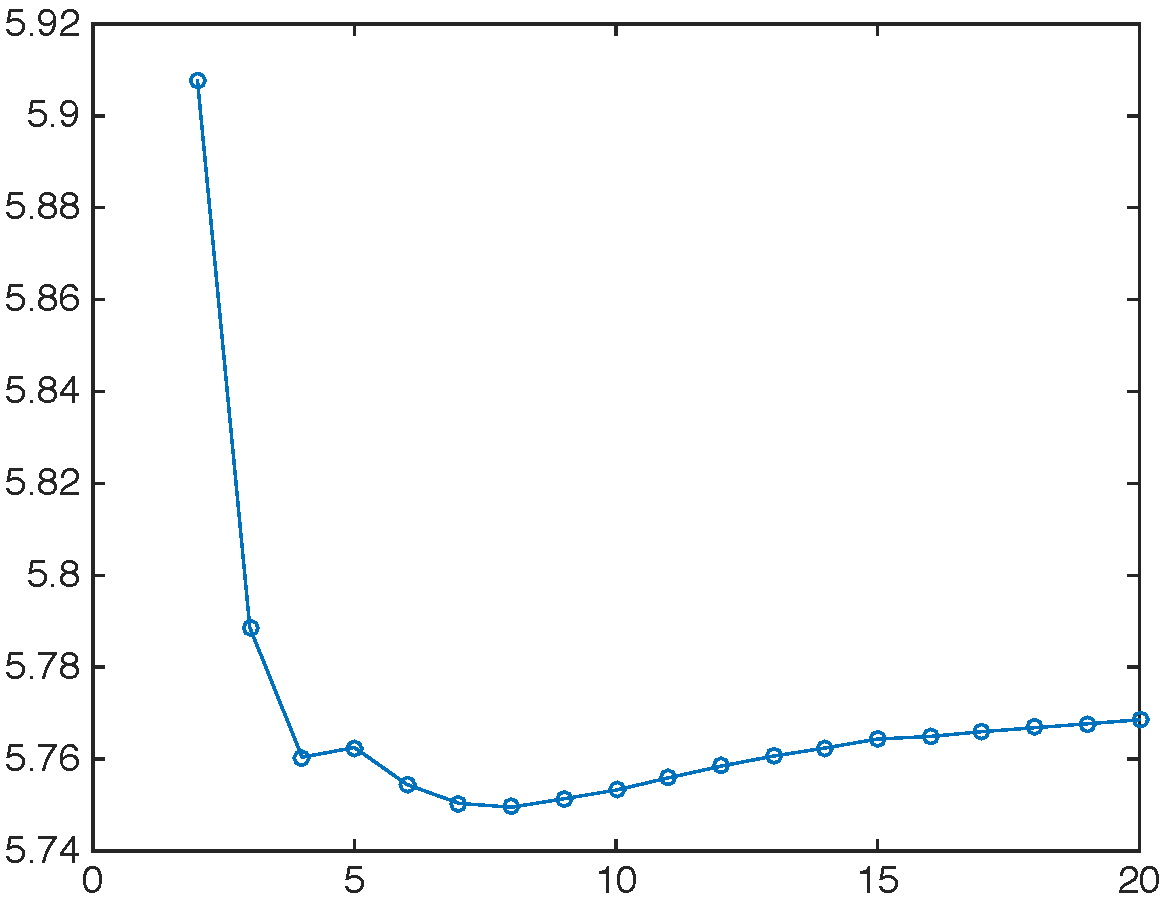
\includegraphics[width=.8\linewidth]{momentsentropy_smpl_30_dataset_thermomech_TCcrop}
%		\caption{Previous MaxEnt Algorithm, Entropy against Moments}
%		\label{fig:previousmaxentmomentsentropy}
%	\end{subfigure}
%	\begin{subfigure}%{.2\textwidth}
%		\centering
%		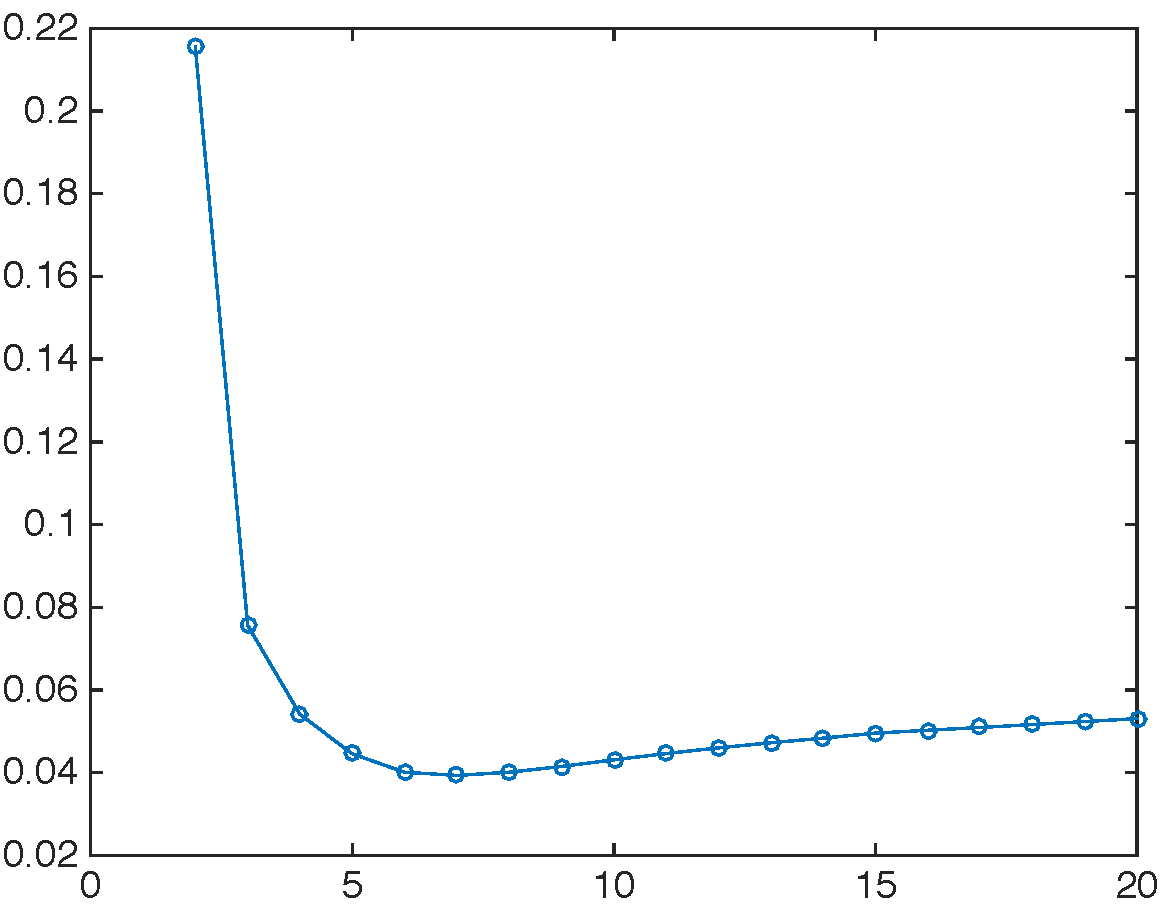
\includegraphics[width=.8\linewidth]{momentserror_smpl_30_dataset_thermomech_TCcrop}
%		\caption{Previous MaxEnt Algorithm, Errors against Moments}
%		\label{fig:previousmaxentmomentserror}
%	\end{subfigure}
%	\begin{subfigure}%{.2\textwidth}
%		\centering
%		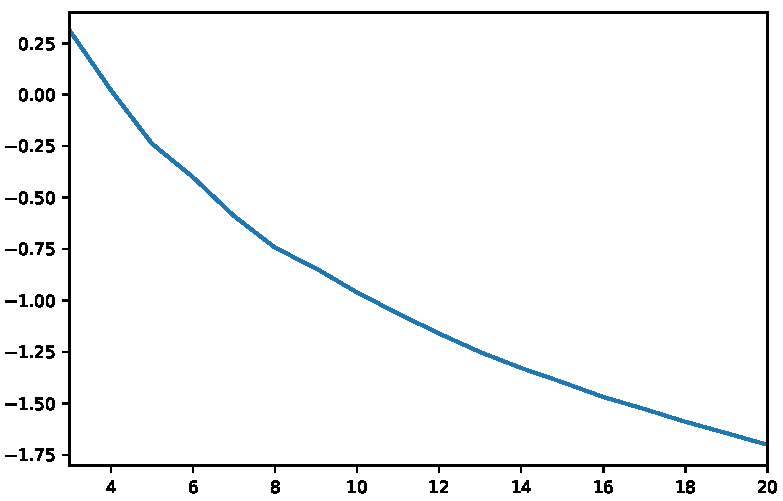
\includegraphics[width=0.9\linewidth]{entropyvsmomentsthermonewcrop}
%		\caption{New MaxEnt Algorithm, Entropy against Moments}
%		\label{fig:newmaxentmomentsentropy}
%	\end{subfigure}
%	\begin{subfigure}%{.2\textwidth}
%		\centering
%		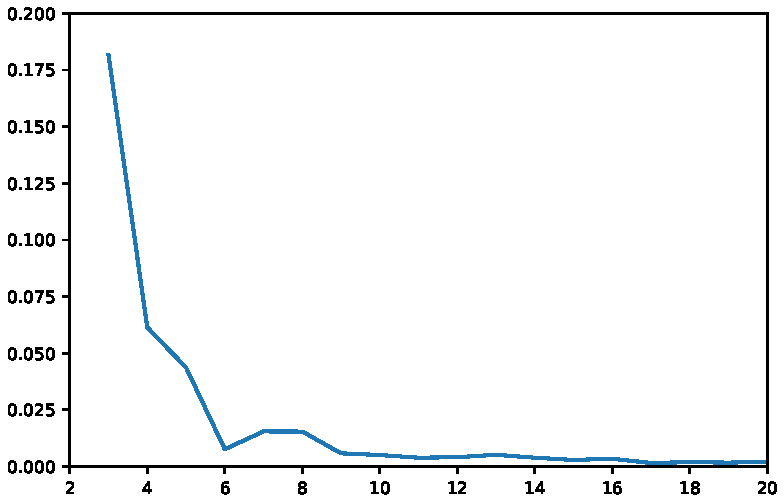
\includegraphics[width=0.9\linewidth]{errorvsmomentsthermonewcrop}
%		\caption{New MaxEnt Algorithm, Error against Moments}
%		\label{fig:newsmaxentmomentserror}
%	\end{subfigure}
%	\caption{New Maximum Entropy Algorithm}
%\end{figure}

\begin{figure}[htp]
	\centering
	\label{figur}\caption{Comparison of Classical and Novel MaxEnt algorithms}
	
	\subfloat[Old Entropy vs Moments]{\label{figur:1}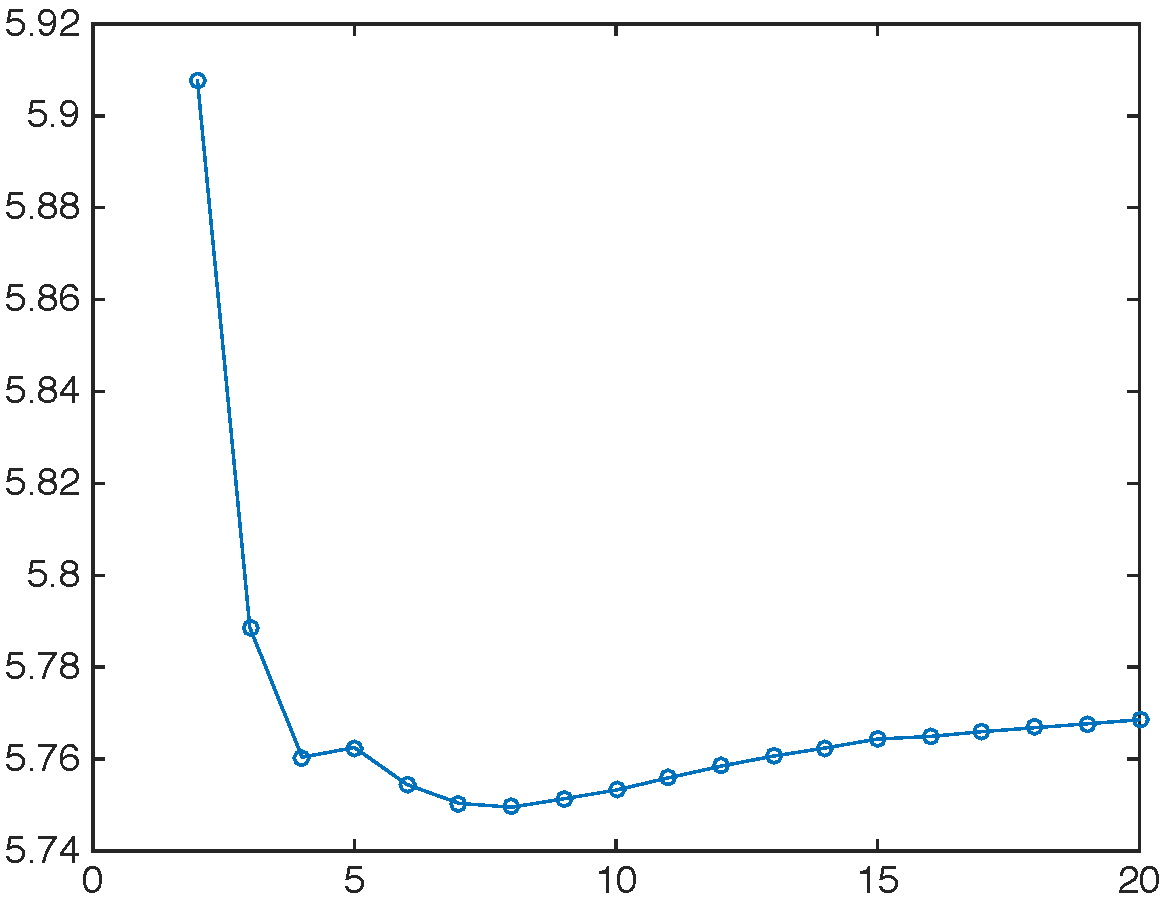
\includegraphics[width=40mm]{momentsentropy_smpl_30_dataset_thermomech_TCcrop}}
	\subfloat[Old Entropy vs Error]{\label{figur:2}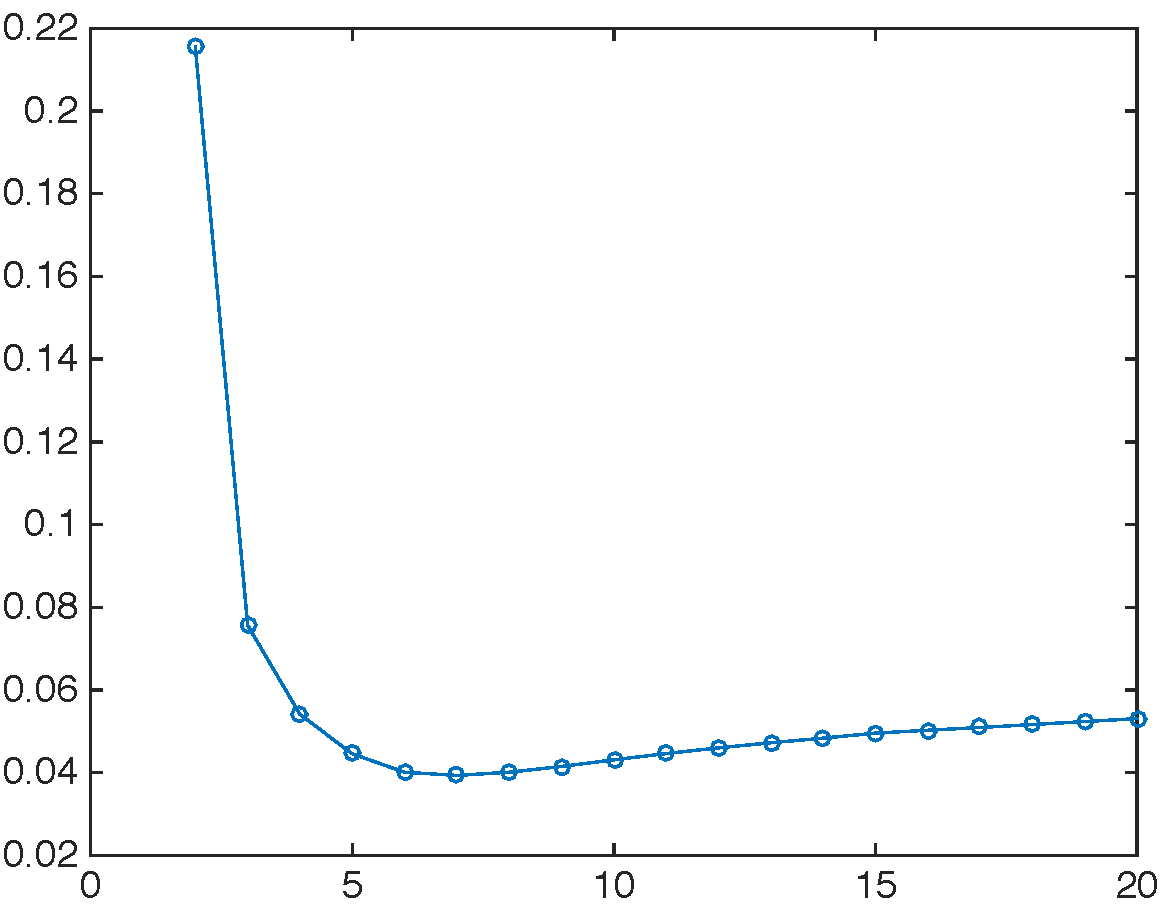
\includegraphics[width=40mm]{momentserror_smpl_30_dataset_thermomech_TCcrop}}
	\\
	\subfloat[New Entropy vs Moments]{\label{figur:3}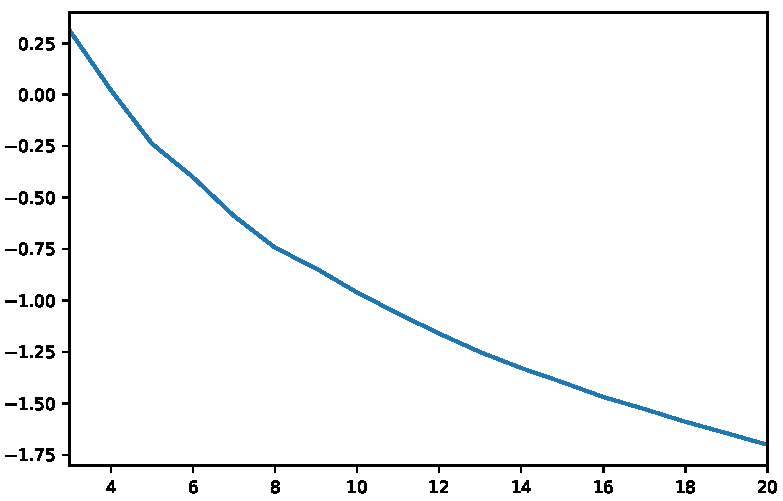
\includegraphics[width=40mm]{entropyvsmomentsthermonewcrop}}
	\subfloat[New Entropy vs Error]{\label{figur:4}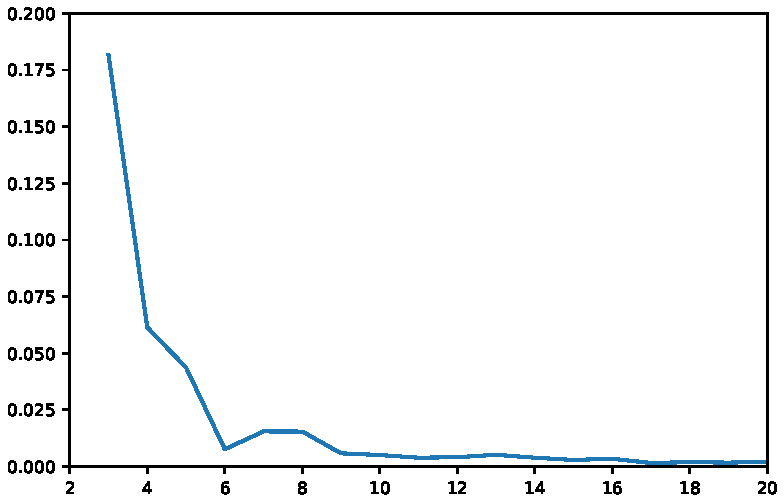
\includegraphics[width=40mm]{errorvsmomentsthermonewcrop}}
	
\end{figure}

\subsection{Synthetic Kernel Data}

We simulate the kernel matrices from a Gaussian/Determinental Point Process \cite{Rasmussen2006}, by generating a typical squared exponential kernel matrix $K \in \mathbb{R}^{n \times n}$ using the Python GPy package with $6$ dimensional, Gaussian inputs. We then add noise of variance $10^{-8}$ along the diagonals. We employ a variety of realistic uniform length-scales. We use $m=30$ Moments, $d=50$ Hutchinson probe vectors and compare our novel MaxEnt algorithm against the Taylor approximation, Chebyshev \cite{han2015large} and Lanczos \cite{ubaru2017fast} in Table \ref{table:errortable}. We see that for low condition numbers (Figure \ref{fig:lscale0.1}) The benefit of framing the log determinant as an optimization problem is marginal, whereas for large condition numbers (Figures \ref{fig:lscale0.33}) the benefits are substantial, with orders of magnitude better results than competing methods. We also provide the number of Chebyshev and Lanczos steps required to achieve similar performance. 
\begin{table}[t]
	\label{table:errortable}
	\caption{Absolute relative error for MaxEnt, Chebyshev \& Lanczos methodson varying length-scale $l$, with varying condition number $\kappa$ on squared exponential kernel matrices $K \in \mathbb{R}^{1000\times 1000}$.}
	\label{sample-table}
	\vskip 0.15in
	\begin{center}
		\begin{small}
			\begin{sc}
				\begin{tabular}{lcccr}
					\toprule
					$\kappa$ & $l$ & MaxEnt & Chebyshev & Lanczos \\
					\midrule
					$3\times10^{1}$    & 0.05& \bf{0.0014}& 0.0037 & 0.0024 \\
					$1.1\times10^{3}$ & 0.15& 0.0522& \bf{0.0104} & 0.0024\\
					$1.0\times10^{5}$    & 0.25& 0.0387& 0.0795 & \bf{0.0072} \\
					$2.4\times10^{6}$    & 0.35& 0.0263& 0.2302    & \bf{0.0196}    \\
					$8.3\times10^{7}$     & 0.45& \bf{0.0284}& 0.3439 & 0.0502\\
					$4.2\times10^{8}$     & 0.55&
					\bf{0.0256}& 0.4089 & 0.0646\\
					$4.3\times10^{9}$     & 0.65&
					\bf{0.00048}& 0.5049 & 0.0838\\
					$1.4\times10^{10}$     & 0.75& \bf{0.0086}& 0.5049  &0.1050       \\
					$4.2\times10^{10}$   & 0.85& \bf{0.0177}& 0.5358 &0.1199\\
					\bottomrule
				\end{tabular}
			\end{sc}
		\end{small}
	\end{center}
	\vskip -0.1in
\end{table}
%\subsection{Sparse Matrices}
%Given that the method described above works in general for any positive definite matrices. We look at large sparse spectral problems. Given that good results are reported for Polynomial methods at even a fairly modest number of moments, we consider very very large sparse matrices, such as social networks\footnote{Facebook, with $10^{9}$ users, each with $\approx 10^{3}$ friends is equivalent to a dense $10^{6}$ matrix}, where we wish to limit the number of non-central moment estimates. We set $m=d=5$ and test on the UFL SuiteSparse dataset. We show our results in table \ref{table2}. VBALD it competitive with Lanczos and we note that similar to the Kernel Matrix case, VBALD does best relative to other methods when the others perform at their poorest, i.e have a relatively large absolute relative error.
%\begin{table}[t]
%	\label{table2}
%	\caption{Absolute relative error for VBALD, Chebyshev \& Lanczos on SuiteSparse Matrices}
%	\label{sample-table}
%	\vskip 0.15in
%	\begin{center}
%		\begin{small}
%			\begin{sc}
%				\begin{tabular}{lcccr}
%					\toprule
%					Dataset & $m$ & VBALD & Chebyshev & Lanczos \\
%					\midrule
%					Thermo    & 5 & $1\times 10^{-2}$& $5\times 10^{-2}$ & $\bf{3\times 10^{-3}}$ \\
%					Water 2    & 5& $4\times 10^{-3}$& $1\times 10^{-2}$ & $\bf{9\times 10^{-4}}$ \\
%					Water 1    & 5& $\bf{2\times 10^{-4}}$& $3\times 10^{-3}$ & $2\times 10^{-4}$ \\
%					jnlbrng1    & 5& $3\times 10^{-2}$& $3\times 10^{-2}$ & $\bf{2\times 10^{-2}}$ \\
%					finan512    & 5& $9\times 10^{-3}$& $8\times 10^{-2}$ & $\bf{1\times 10^{-3}}$ \\
%					
%					Ecology 2    & 5& $\bf{1\times 10^{-2}}$& $1\times 10^{-2}$ & $3\times 10^{-2}$ \\
%					Apache    & 5& $\bf{5\times 10^{-2}}$& $2\times 10^{-2}$    & $8\times 10^{-2}$    \\
%					
%					
%					\bottomrule
%				\end{tabular}
%			\end{sc}
%		\end{small}
%	\end{center}
%	\vskip -0.1in
%\end{table}

\section{Machine Learning Application 1: DPPs}
Determinantal point processes (DPPs) \cite{macchi1975coincidence} are probabilistic models capturing global negative correlations. %They describe Fermions \footnote{as a consequence of the spin-statistics theorem} in Quantum Physics, Eigenvalues of random matrices and non-intersecting random walks. 
In machine learning their natural selection of diversity has found applications in the field of summarization \cite{gong2014diverse}, human pose detection \cite{kulesza_2012}, clustering \cite{kang2013fast}, Low rank kernel matrix approximations \cite{li2016fast} and Manifold learning \cite{wachinger2015sampling}. Formally, it defines a distribution on $2^{y}$, where $y = [n]$ is the finite ground set. For a random variable $X \subseteq Y$ drawn from a given DPP we have
\begin{equation}
P(X = x) \propto \mathrm{det}(K_{X}) = \frac{\mathrm{det}(K_{x})}{\mathrm{det}(K+I)},
\end{equation}
where $K \in 
{R}^{d\times d}$ is a positive definite matrix referred to as the $L$-ensemble kernel. Greedy algorithms that find the most diverse set $Y$ of $y$ that achieves the highest probability, i.e $\mathrm{argmax}_{X\subseteq y} \mathrm{det}(K_{Y})$ require the calculation of the marginal gain, 
\begin{equation}
\log \mathrm{det} K_{X\cup\{i\}} - \log \mathrm{det} L_{X}.
\end{equation}
%with $\mathcal{O}(n^{3})$ computational complexity. Previous work has looked at limiting the burden of the computational complexity by employed Chebyshev approximations to the Log Determinant \cite{han2017faster}. However their work is limited Kernel Matrices with minimum eigenvalues of $10^{-3}$\footnote{or alternatively low condition numbers}, which does not cover the class of realistic kernel matrix spectra, notably the popular squared exponential kernel. We develop a method in section \ref*{method} and an algorithm \ref{algorithm} which is capable of handling very high condition numbered matrices.
{\color{red}{ADD DPP EXPERIMENT HERE}}





%%%%%%%%%%%%%%%%%%%%%%%%%%%%%%%%%%%%%%%%%%%%%%%%%%%%%%%
%%%%%%%%%%%%%%%%%%   Motivating Example for clustering %%%%%%%%%%%%%%%%%%%%%%
%%%%%%%%%%%%%%%%%%%%%%%%%%%%%%%%%%%%%%%%%%%%%%%%%%%%%%%

\section{Machine Learning Application 2: Learning Cluster Number}
For many clustering algorithms, the number of clusters is taken as a given input 
%check the second one here, that k really is an input
\cite{liu2013large},\cite{cucuringu2016simple}
%check the second one here, that k really is an input
The estimation of the cluster number is a challenging problem, \citep{von2007tutorial}, with likelihood, ad-hoc, information theoretic, stability and spectral approaches advocated. In the latter, one analyses the spectral gap in the eigenvalue spectrum, which we refer to as \emph{eigengap} for short. %Applying this approach in the era of big-data (where social networks such as Facebook are approaching $n = 2\times 10^9$ users) means that standard approaches, such as the canonical Cholesky decomposition, with computational complexity $\mathcal{O}(n^{3})$  and storage $\mathcal{O}(n^{2})$ are completely prohibitive. 
The Lancsoz algorithm, which exploits matrix sparsity by working with matrix vector multiplications,  has computational complexity $\mathcal{O}(n_\mathrm{nz}\times m + nm^{2})\times d$, where for very large sparse matrices, the second term becomes dominant. Given that empirically many social, biological and technical communities are sparse and that all we need for detecting cluster count is an estimation of the eigenvalues and not the eigenvectors, we look for an alternative computationally more effective method of estimating the spectral density. We use the method of maximum entropy, with computational complexity equivalent to Lancsoz without the second term. 
%\subsection{Related Work} 
%\label{relatedwork}
%Krylov subspace methods, using matrix vector products, such as the Lanczos algorithm have been applied to estimating eigengaps and detecting communities with encouraging results \citep{{ubaruapplications},{kang2011spectral}}.
%The computational complexity of the Lanczos algorithm is $\mathcal{O}(n_\mathrm{nz}\times m + nm^{2})\times d$, where $n$ is the rank of the square matrix $M \in \mathbb{R}^{n\times n}$,
%$d$ the number of random starting vectors used and $m$ the number of Lanczos steps taken. 
%The computational complexity of our Entropic Spectral Learning is $\mathcal{O}(n_\mathrm{nz}\times m)\times d$, where $m$ is the number of moments used, this is a lower computational complexity than Lacnsoz, as there is no need to orthogonalize and store the vectors at each step. The second Lanczos term dominates at $m > n_\mathrm{nz}/n$. For many networks in the Stanford Large Network Dataset Collection (SNAP) \citep{snapnets}, such as Amazon, YouTube, Wikipedia and LiveJournal, this condition is reached for low values of $m$: respectivley, $3,3,14,6$.

%%%%%%%%%%%%%%%%%%%%%%%%%%%%%%%%%%%%%%%%%%%%%%%%%%%%%%%
%%%%%%%%%%%%%%%%%%   Graph Notation  %%%%%%%%%%%%%%%%%%%%%%
%%%%%%%%%%%%%%%%%%%%%%%%%%%%%%%%%%%%%%%%%%%%%%%%%%%%%%%

%\subsection{GRAPH NOTATION }
%Graphs are the mathematical structure underpinning the formulation of networks. Let $G = (V,E)$ be an undirected graph with vertex set $V = \{v_{1},...,v_{N}\}$. Each edge between two vertices $v_{i}$ and $v_{j}$ carries a non-negative weight $w_{ij}>0$ and $w_{ij}=0$ corresponds to two disconnected nodes. For un-weighted graphs we set $w_{ij}=1$ for two connected nodes. The \textit{adjacency matrix} is defined as $W = (w_{ij})$ with $i,j=1,...,n$. The degree of a vertex $v_{i} \in V$ is defined as 
%\begin{equation}
%d_{i} = \sum_{j=1}^{n}w_{ij}.
%\end{equation}
%The \textit{degree matrix} $D$ is defined as a diagonal matrix that contains the degrees of the vertices along diagonal, i.e., $D_{ii} = d_{i}$ and zero otherwise. The \textit {unnormalised graph Laplacian matrix} is defined as
%\begin{equation}
%L = D - W.
%\end{equation}
%As $G$ is undirected, i.e., $w_{ij}=w_{ji}$, the adjacency, degree and unnormalised Laplacian matrices are all symmetric. This ensures that the eigenvalues of the Laplacian are real. Another common variant of the Laplacian matrix is the so-called \textit{normalised graph Laplacian}  \citep{chung1997spectral}
%\begin{eqnarray}
%\tilde{L} &=& D^{-1/2}LD^{-1/2}  \nonumber\\
%&=& I - \tilde{W} = I - D^{-1/2}WD^{-1/2}\label{lnorm},
%\end{eqnarray}
%where $\tilde{W}$ is known as the normalised adjacency matrix\footnote{Strictly speaking, the second equality only holds for graphs without isolated vertices.}. For our analysis we will be using the Laplacian matrix. 

%Notice that for regular graphs where all the vertices have the same degree, there is no commonly adopted convention on which Laplacian to use as all Laplacians are similar to each other \citep{von2007tutorial}, but outside of this regime the different variants of the Laplacians may vary considerably. For our experiments we use the normalised Laplacian.%, alternatively we could have used the unnormalised Laplacian and divided by the Gershgorin bound \citep{gershgorin1931uber} or the number of nodes $n$.

%%%%%%%%%%%%%%%%%%%%%%%%%%%%%%%%%%%%%%%%%%%%%%%%%%%%%%%
%%%%%%%%%%%%%%%%%%   Graph Eigenstructure  %%%%%%%%%%%%%%%%%%%%%%
%%%%%%%%%%%%%%%%%%%%%%%%%%%%%%%%%%%%%%%%%%%%%%%%%%%%%%%

%\section{Graph Eigenstructure}
%Isomorphic graphs are co-spectral. This means that any relabelling of node numbers has no effect on their adjacency matrices after a permutation of rows and columns. Spectral techniques have been used extensively to characterise global network structure \citep{newman2006modularity} and in practical applications thereof, such as facial recognition/computer vision \citep{belkin2003laplacian}.
%Whilst there exist non-isomorphic cospectral graphs, such as the Saltire pair, computer simulations show that beyond $n\geq9$ vertices, the fraction $f$ of graphs with co-spectral adjacency and Laplacian matrices decreases and it is conjectured that for $n\rightarrow\infty$ that $f\rightarrow 0$. Furthermore the spectrum of the adjacency and the Laplacian matrices can be used to deduce important quantities, such as the number of vertices and edges, where the graph is regular (fixed girth) or bipartite, the number of closed walks, the number of components and the number of spanning trees \citep{van2003graphs}.


%%%%%%%%%%%%%%%%%%%%%%%%%%%%%%%%%%%%%%%%%%%%%%%%%%%%%%%
%%%%%%%%%%%%%%  Clustering using  Eigenspectra  %%%%%%%%%%%%%%%%%%%%%%
%%%%%%%%%%%%%%%%%%%%%%%%%%%%%%%%%%%%%%%%%%%%%%%%%%%%%%%


\subsection{CLUSTERING USING THE EIGENSPECTRA}
%We reproduce the result that the multiplicity of zero eigenvalues for the graph $G$ indicates its number of connected components. We then use matrix perturbation theory and the Cauchy-Schwarz inequality to show that by adding a small number of edges between the connected components, these eigenvalues are perturbed by a small positive amount. Hence if this perturbation is small compared to the original spectral gap, we can still determine the number of clusters by integrating the spectral density until the first minimum and then multiplying by the dimension of the Laplacian matrix. The following result is well known (\cite{von2007tutorial}).
%\begin{proposition}
%\label{numberof0eigenvalues}
%Let G be an undirected graph with non-negative weights. Then the multiplicity $k$ of the eigenvalue $0$ of the Laplacian $L\in \mathcal{R}^{n\times n}$ is equal to the number of connected components $A_{1},...,A_{k}$ in the graph. The eigenspace of the eigenvalue $0$ is spanned by the indicator vectors $\mathbbm{1}_{A_{1}},....,\mathbbm{1}_{A_{k}}$.
%\end{proposition} 
%For completeness we outline the proof here. Note that, by the definition of the unnormalised Laplacian, we have $L_{ij} = \mathbbm{1}_{i=j}\sum_{k=1}^{n}w_{ik}-w_{ij}$ and hence if we set $u_{j} = 1$ with $u_{j}$ being the $j$-th element of $\mathbf{u}$,=
%\begin{equation}
%\lambda \times u_{i} = \sum_{j=1}L_{ij}u_{j} = \sum_{j=1}\bigg(- w_{ij}+\mathbbm{1}_{i=j}\sum_{k=1}w_{ik}\bigg) = 0 
%\end{equation}
%This proves that the vector $\mathbf{u} = [1,....,1]^T$ is an eigenvector with eigenvalue $\lambda = 0$. For $k$ connected components, the matrix $L$ has a block diagonal form
%\[
%L = \begin{bmatrix}
%L_{1} & 0  &\dots  & 0\\
%0 & L_{2} & \ddots  & \vdots\\
%\vdots & \ddots & \ddots & 0\\
%0 & \dots & 0 & L_{k}
%\end{bmatrix}
%\]
%As is the case for all block diagonal matrices, the spectrum of $L$ is given by the union of the spectra $L_{i}$. From the proceeding we know that every Laplacian $L_{i}$ has an eigenvalue $0$ with multipicity $1$, hence $L$ has eigenvalue $0$ with multiplicity $k$ and corresponding eigenvectors of $L$ are those of $L_{i}$ filled with $0$ at the positions of the other blocks.

It is well known \cite{von2007tutorial}, that the multiplicity of the $0$ eigenvalues is equal to the number of disconnected components in the graph. Hence were we to define a community as a completely disconnected component, we could simply count the number of $0$ eigenvalues. However given that real world networks are rarely completely disconnected, this procedure would be of little practical utility. We hence consider groups of nodes containing far greater intra-group connections than inter-group connections as well defined clusters. %This conforms to our natural intuition of a group or community.  
If the graph is connected, but consists of $k$ subgraphs which are ``weakly'' linked to each other, the graph Laplacian has one zero eigenvalue and all the other eigenvalues positive. 
This is easily seen by looking at
\begin{equation}
\mathbf{u}^{T}L \mathbf{u} = \sum_{i,j=1}^{n}w_{ij}(u_{i}-u_{j})^{2}
\end{equation}
which is positive, as $w_{ij}>0$ and given a connected graph $G$ has a single $0$ eigenvalue, all other eigenvalues are thus positive. For small changes in the Laplacian, we expect from matrix perturbation theory \citep{bhatia2013matrix} that the next $k-1$ smallest eigenvalues will be close to $0$. Hence, given the spectral decomposition, the number of eigenvalues very close to $0$ corresponds to the number of clusters. 
\subsubsection{Estimating the Cluster Number using Maximum Entropy:}
For any smoothed spectral density, which we learn using stochastic trace estimation (Section \ref{stochastictrace}) and MaxEnt (Algorithm \ref{alg:maxent}), to count the number of near $0$ eigenvalues, one simply integrates the spectral density until the first spectral minimum (found using gradient descent) and then multiplies by number of Nodes $N$, we illustrate this in Algorithm \ref{alg:clusteralg}.


%\subsection{Analytical forms for the Differential Entropy and Divergence from MaxEnt}
%In other work using either the exact eigen-decomposition \citep{takahashi2012discriminating} or Chebyshev/Lanczos \citep{ubaruapplications} as the differential entropy of delta function
%\begin{equation}
%\mathcal{S}(\delta(x)) = 1/2 \log(2\pi e\sigma^{2}) \xrightarrow{\sigma\rightarrow 0} -\infty .
%\end{equation}
%Gaussian Kernel regression, along with a prescriptions for the Bandwidth using the Sturges criterion is used. Given that neither the differential entropy of a Gaussian mixture nor the Kullback-Leiber/Shannon-Jensen divergence between a Gaussian mixture has an analytical form \citep{hershey2007approximating}, this too must be approximated using either Monte-Carlo sampling or numerical quadrature. An advantage of the Maximum Entropy formalism is that both can be calculated trivially after having completed the optimisation.
%To calculate the differential entropy we simply note that
%\begin{equation}
%\mathcal{S}(p) = \int p(\lambda) (1+\sum_{i}^{m}\alpha_{i}x^{i}) d\lambda= 1+\sum_{i}^{m}\alpha_{i}\mu_{i}
%\end{equation}
%where $p(\lambda) = \exp[-(1+\sum_{i}^{m}\alpha_{i}x^{i})]$.
%
%
%The KL divergence between two Maximum Entropy spectra, $p(\lambda) = \exp[-(1+\sum_{i}\alpha_{i}x^{i})]$ and $q(\lambda) = \exp[-(1+\sum_{i}\beta_{i}x^{i})]$, can be written as
%\begin{equation}
%\mathcal{D}_{kl}(p||q) = \int p(\lambda) \log \frac{p(\lambda)}{q(\lambda)}d\lambda = -\sum_{i}(\alpha_{i}-\beta_{i})\mu_{p}^{i},
%\end{equation}
%where $\mu_{p}^{i}$ refers to the $i$-th moment constraint of the density $p(\lambda)$. Similarly the Jensen-Shannon divergence can be written as 
%\begin{equation}
%\frac{\mathcal{D}_{kl}(p||q)+\mathcal{D}_{kl}(q||p)}{2} = \frac{\sum_{i}(\alpha_{i}-\beta_{i})(\mu_{q}^{i}-\mu_{p}^{i})}{2},
%\end{equation}
%where all the $\alpha_{i}$ and $\beta_{i}$ are derived from the optimisation and the $\mu$'s are given from the stochastic trace estimation.

%%%%%%%%%%%%%%%%%%%%%%%%%%%%%%%%%%%%%%%%%%%%%%%%%%%%%%%
%%%%%%%%%%%%%%%%%%%  EXPERIMENTS  %%%%%%%%%%%%%%%%%%%%%%%
%%%%%%%%%%%%%%%%%%%%%%%%%%%%%%%%%%%%%%%%%%%%%%%%%%%%%%%

\section{Experiments}
\label{experimentsgraph}
We follow the experimental setup in Section \ref{experiments}, use $d=100$ Gaussian random vectors for our stochastic trace estimation, for both MaxEnt and Lanczos \citep{ubaru2017fast}. 
%We explain the procedure of going from Adjacency matrix to Laplacian moments in Algorithm \ref{alg:preprocessing}. 
When comparing MaxEnt with Lanczos we set the number of moments $m$ equal to the number of Lanczos steps%, as they are both matrix vector multiplications in the Krylov subspace. We implement a quadrature MaxEnt algorithm \ref{alg:maxent}.
%We use a grid size of $10^{-4}$ over the interval $[0,1]$ and add diagonal noise on the Hessian to improve conditioning and symmetrise it. We further use Chebyshev polynomial input instead of power moments for improved performance and conditioning. 
In order to normalise the moment input we use the normalised Laplacian with eigenvalues bounded by $[0,2]$ and divide by $2$. 
%We use Python's Scipy implementation of the Newton conjugate gradient algorithm (\cite{scipy}) for the MaxEnt Lagrange multipliers. 
%We then apply our cluster estimator, Algorithm \ref{alg:clusteralg} to both the spectral density derived from our MaxEnt implementation and to that implied by the Lancsoz algorithm. 
To make a fair comparison we take the output from Lancsoz \citep{ubaru2017fast} and apply kernel smoothing \citep{lin2016approximating} before applying our cluster estimator. We explain the details of our kernel smoothing in section \ref{smoothinglancsoz}.

%\begin{algorithm}[tb]
%	\caption{Learning the Graph Laplacian Moments}
%	\label{alg:preprocessing}
	
%	\begin{algorithmic}[1]
%		\STATE {\bfseries Input:} Normalized Laplacian $\{\tilde{L}\}$, Number of Probe Vectors $d$, Number of moments required $m$
%		\STATE {\bfseries Output:} Moments of Normalised Laplacian $\{\mu_{i}\}$
%		\FOR {$i$ in $1,..,d$}
%		\STATE  Initialise random vector $\vec{z}_{i}\in R^{1\times n}$
%		\FOR {$j$ in $1,..,m$}
%		\STATE $\vec{z_{i}}' = \tilde{L}\vec{z}_{i}$
%		\STATE $\rho_{i,j} =  \vec{z}_{i}^{T}\vec{z_{i}}'$
%		%\STATE $j = j+1$
%		\ENDFOR
		%\STATE $$
%		\ENDFOR
%		\STATE $\mu_{i} = 1/d \times \sum_{j=1}^{d}\rho_{i,j}$ 
%		%\UNTIL{$noChange$ is $true$}
%	\end{algorithmic}
%\end{algorithm}

\begin{algorithm}[tb]
	\caption{MaxEnt Algorithm}
	\label{alg:maxent}
	
	\begin{algorithmic}[1]
		\STATE {\bfseries Input:} Moments $\{\mu_{i}\}$, Tolerance $\epsilon$, Hessian noise $\eta$
		\STATE {\bfseries Output:} Coefficients $\{\alpha_{i}\}$
		\STATE Initialize $\alpha_{i} = 0$.
		\STATE Minimize $\int_{0}^{1}p_{\alpha}(\lambda)d\lambda + \sum_{i}\alpha_{i}\mu_{i}$
		\STATE Gradient $\mu_{j}-\int_{0}^{1}p_{\alpha}(\lambda)\lambda^{j}d\lambda$
		\STATE Hessian  $ = \int_{0}^{1}p_{\alpha}(\lambda)\lambda^{j+k}d\lambda$
		\STATE Hessian $= (H+H')/2 + \eta$
		\STATE Until $\forall j$ Gradient$_{j} < \epsilon$		
		%\UNTIL{$noChange$ is $true$}
	\end{algorithmic}
\end{algorithm}
\begin{algorithm}[tb]
	\caption{Cluster Estimator Algorithm}
	\label{alg:clusteralg}
	
	\begin{algorithmic}[1]
		\STATE {\bfseries Input:} Lagrange Multipliers ${\alpha_{i}}$, Matrix Dimension $n$, Tolerance $\epsilon$
		\STATE {\bfseries Output:} Number of Clusters $N_{c}$
		\STATE Initialize $p(\lambda) \rightarrow p(\lambda|\alpha_{i}) = \exp{-[1+\sum_{i}\alpha_{i}x^{i}]}$.
		%How shall we write this bit??
		\STATE Minimize $\lambda*$ s.t $\frac{dp(\lambda)}{d\lambda}|_{\lambda=\lambda*} \leq \epsilon$
		\STATE Calculate $N_{c} = n\int_{0}^{\lambda*} p(\lambda)d\lambda$	
		%\UNTIL{$noChange$ is $true$}
	\end{algorithmic}
\end{algorithm}

\begin{algorithm}[tb]
	\caption{Stochastic Trace Estimation}
	\label{alg:stochtrace}
	
	\begin{algorithmic}[1]
		\STATE {\bfseries Input:} Number of Random Vectors $d$, Number of Moments $m$, Matrix $M^{n\times n}$
		\STATE {\bfseries Output:} Moment Expectations $\mathbb{E}_{\mu}(\lambda^{i})$ $\forall i\leq m$
	\STATE {Initialize $\mathbb{E}_{\mu}(\lambda^{i}) = 0$ $ \forall i$} 	
	 \FOR{$i \leq d$} \STATE {Initialize $\vec{z}_{d} = rand(1,n) $} 
		 \FOR{$j \leq m$} \STATE {$\vec{z}_{d} = M*\vec{z}_{d}$} 
		 \STATE {$\mathbb{E}_{\mu}(\lambda^{j}) = \mathbb{E}_{\mu}(\lambda^{j}) + \frac{1}{d} \vec{z}_{d}^{t}*\vec{z}_{d}$ }
		 \ENDFOR
	 \ENDFOR
	\end{algorithmic}
\end{algorithm}



\subsection{Synthetic Data}
In order to test the robustness of the approach to networks with clusters of different structures, we implement a mixture of Erd{\"o}s-R{\'e}nyi , Watts-Strogatz and Barabási-Albert networks using the Python package \textit{NetworkX} and conduct multiple experiments using networks that have from $9$ to $240$ clusters, with each cluster containing $30$ nodes. We connect the nodes between clusters randomly, with a single inter-cluster connection. We show the results in Table \ref{table:clustererrortable}.






\begin{table}[t]
	\label{table:clustererrortable}
	\caption{Fractional error in community detection for synthetic networks using MaxEnt and Lanczos with 80 moments}\label{table:fractional_error_syn}
	\begin{center}
		\begin{small}
			\begin{sc}
				\begin{tabular}{lcccr}
					\toprule
					\# of clusters (n) & Lanczos  & MaxEnt \\
					\midrule
					9 (270)    & $ \mathbf{3.20 \times 10^{-3}}$   & $9.70 \times 10^{-3}$  \\
					%15 (450)  & $ \mathbf{5.19 \times 10^{-2}}$   & $6.50\times 10^{-2}$   \\
					30 (900) & $ 1.41\times 10^{-2}$   & $ \mathbf{6.40 \times 10^{-3}}$ \\
					%60 (1800) & $4.53\times 10^{-2}$   & $\mathbf{1.50\times 10^{-3}}$   \\
					90 (2700) & $1.81\times 10^{-2}$   & $\mathbf{5.80\times 10^{-3}}$   \\
					%120 (3600) & $\mathbf{1.57\times 10^{-2}}$   & $1.60\times 10^{-2}$   \\
					240 (7200) & $2.89\times 10^{-2}$   & $\mathbf{3.50\times 10^{-3}}$   \\
					\bottomrule
				\end{tabular}
			\end{sc}
		\end{small}
	\end{center}
	\vskip -0.1in
\end{table}

%Figure \ref{fig:synnetwork} shows the community detection errors, expressed in the logarithm to the base 10, for networks of $9$, $30$, $90$, $240$ clusters over number of matrix vector calculations (i.e. number of moments).  We see that for both methods, the detection error generally decreases as more moments are used. For an equivalent number of matrix vector calculations, MaxEnt outperforms the Lanczos algorithm. As there is no accepted prescription by which we can determine when the spectral minimum has been best learned, the occasional dips in error produced by Lanczos (such as for $15$ moments in Figure \ref{fig:sub4} are unlikely to be replicated in real world experiments. 

%Table \ref{table:fractional_error_syn} displays the fractional errors in community detection when we apply Lanczos and MaxEnt, both using 80 moments, to synthetic networks of different sizes and cluster numbers. In each case, lower detection error is highlighted in bold. It is evident that MaxEnt outperforms Lanczos as the number of clusters and the network size increase. 
%We observe a general improvement in performance for larger graphs, visible in the differences between fractional errors for MaxEnt and not Lanczos. This is to be expected as the true spectral density
%\begin{equation}
%p(\lambda) = \frac{1}{n}\sum_{i}^{n}\delta(\lambda-\lambda_{i})
%\end{equation}
%becomes continuous in the $n\rightarrow\infty$ limit and hence we expect the density to be better approximated by a continuous distribution for larger $n$ \citep{ete}. %There are also arguments from the information theoretic literature which state that for macroscopic systems (large $n$), the distribution of maximum entropy dominates the space of solutions for the given constraints \citep{fluctuationpriors}. Essentially this means that for larger and larger systems, assuming that we have incorporated the correct constraints, which for spectral density estimation stochastic trace constraints do (\cite{DBLP:conf/bigdataconf/GranziolR17}) the true distribution looks more and more like that of maximum entropy. Furthermore other distributions, i.e a particular realization of Gauss-Lancsoz quaderature (\cite{ubaru2017fast}) becomes increasingly unlikely. 
%\\\\
To test the performance of our approach for networks that are too big to apply eigen-decomposition, we also generate two large networks by mixing Erd{\"o}s-R{\'e}nyi, Watts-Strogatz and Barabási-Albert networks. The first large network has a size of  201,600 nodes and comprises 350 interconnected clusters whose size varies from 500 to 1000 nodes. The other large network has a size of 404,420 nodes and comprises interconnected 1355 clusters whose size varies from 200 to 800 nodes. The results in Figure \ref{fig:largeSyntheNet} show that our MaxEnt approach outperforms Lanczos for both large synthetic networks.

\begin{figure}
	\centering
	\begin{subfigure}
		\centering
		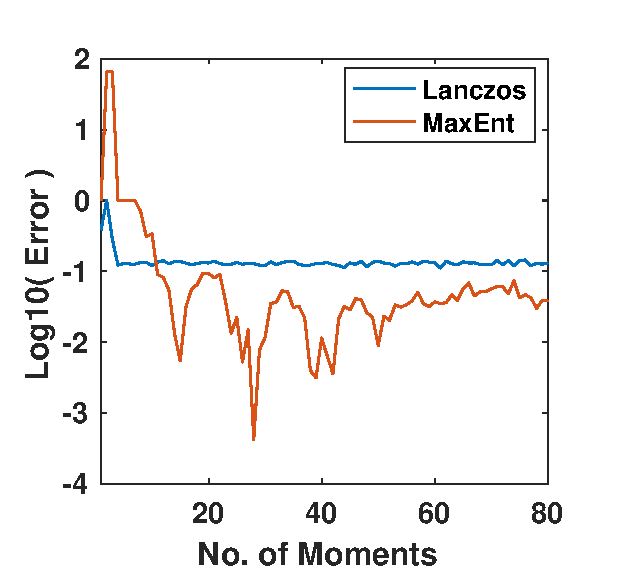
\includegraphics[trim=0cm 0cm 0.1cm 0.0cm, clip, width=1.0\linewidth]{Figures/SynNet_n=201600_c=305.eps}
		\caption{305 clusters}
		\label{subfig:emailerror1}	
	\end{subfigure}%
	\begin{subfigure}
		\centering
		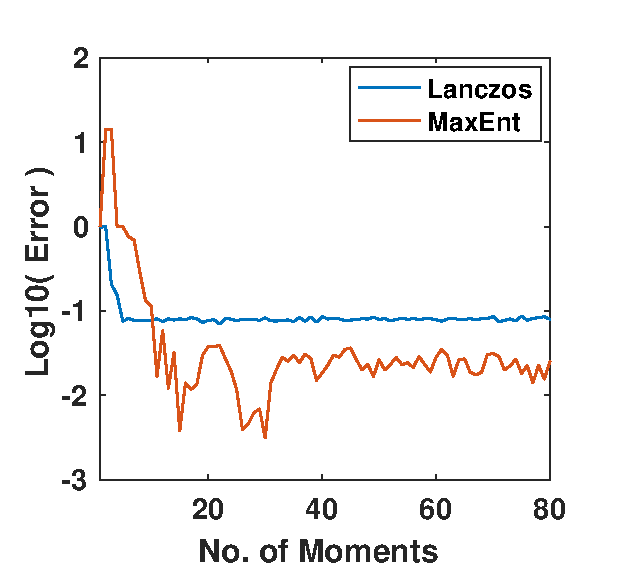
\includegraphics[trim=0cm 0cm 0.1cm 0.0cm, clip, width=1.0\linewidth]{Figures/SynNet_c_1355_n_404420.eps}
		\caption{1,355 clusters}
		\label{subfig:emailerror2}	
	\end{subfigure}%
	\caption{Log error of community detection using MaxEnt and Lanczos on large synthetic networks: a) synthetic network of  201,600 nodes and 305 clusters and b) synthetic network of 404,420 nodes and 1,355 clusters.}
	\label{fig:largeSyntheNet}	
\end{figure} 

%\subsection{Real Data}

\subsubsection{Small Real World Data}
%\begin{figure}
%	\centering
%	\begin{subfigure}
%		\centering
%		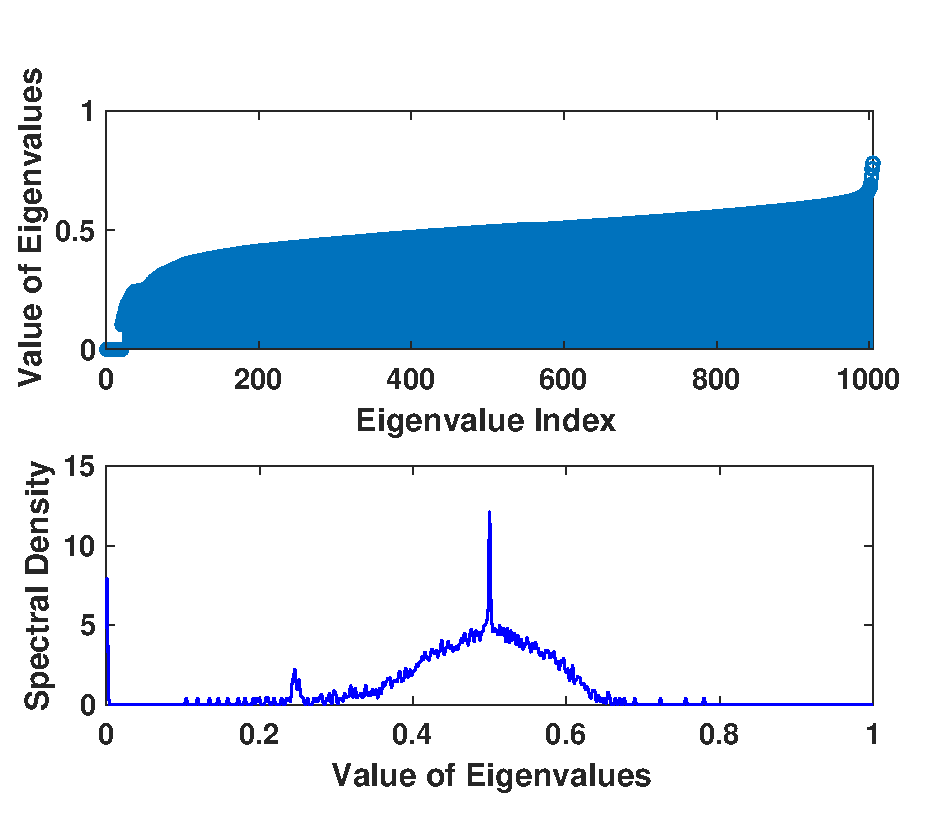
\includegraphics[trim=0cm 0cm 0.1cm 0.8cm, clip, width=1.0\linewidth]{Figures/Stem_Density_Email.eps}
%		\caption{Stem Graph and Eigen-Spectrum}
%		\label{subfig:emailerror1}	
%	\end{subfigure}%
%	
%	\begin{subfigure}
%		\centering
%		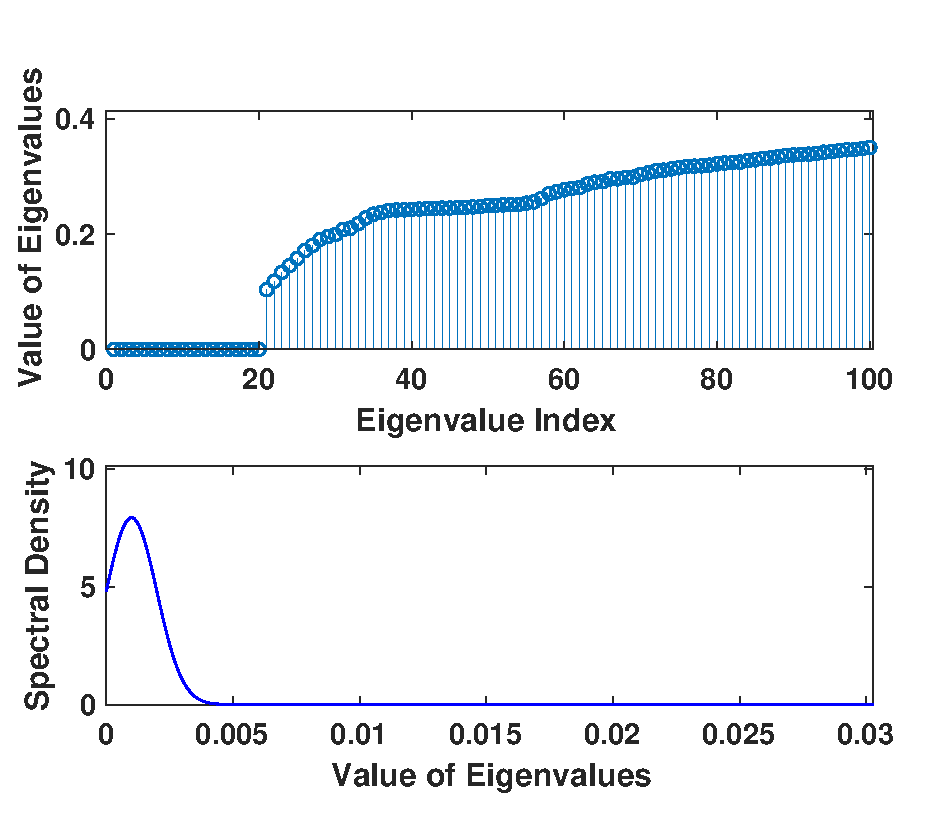
\includegraphics[trim=0cm 0cm 0.1cm 0.8cm, clip, width=1.0\linewidth]{Figures/Stem_Density_Email2.eps}
%		\caption{Zoomed-in Graphs}
%		\label{subfig:emailerror2}	
%	\end{subfigure}%
%	\caption{Stem graph of the eigen-spectrum of the Email Dataset. The subplot $(a)$ shows all the eigenvalues and the whole eigenvalue spectrum. The subplot $(b)$ is a zoomed-in version of $(a)$, which displays the smallest 100 eigenvalues with a clear spectral gap at 20 and the corresponding spectral density near the origin. The area under the spectral density up to 0.005 multiplied by the number of nodes $n$ predicts the number of clusters.}
%	\label{fig:email}	
%\end{figure} 

When the number of nodes $n \approx 10^{3}$, it is possible to compute the eigen-decomposition exactly and hence to benchmark the performance of our algorithm in the real world. 

The first real-world dataset we use is the Email network, which is generated using email communication data among $1,005$ members of a large European research institution and is an undirected graph of $n=1,005$ nodes. We calculate the ground-truth by computing the eigenvalues explicitly and finding the spectral gap near $0$. %As shown in Figure \ref{fig:email}, we count $20$ very small eigenvalues before a large jump in magnitude and set this as the ground truth for the number of clusters in the network. This corresponds to a drop in spectral eigendensity as displayed in the lower subplot of Figure \ref{fig:email}. 
We note that this differs from the value of $42$ given by the number of departments at the research institute. A likely reason for this ground truth inflation is that certain departments, Astrophysics, Theoretical Physics and Mathematics for example, may collaborate to such an extent that their division in name may not be reflected in terms of node connection structure.


\begin{figure}[t]
	\centering
	\begin{subfigure}
		\centering
		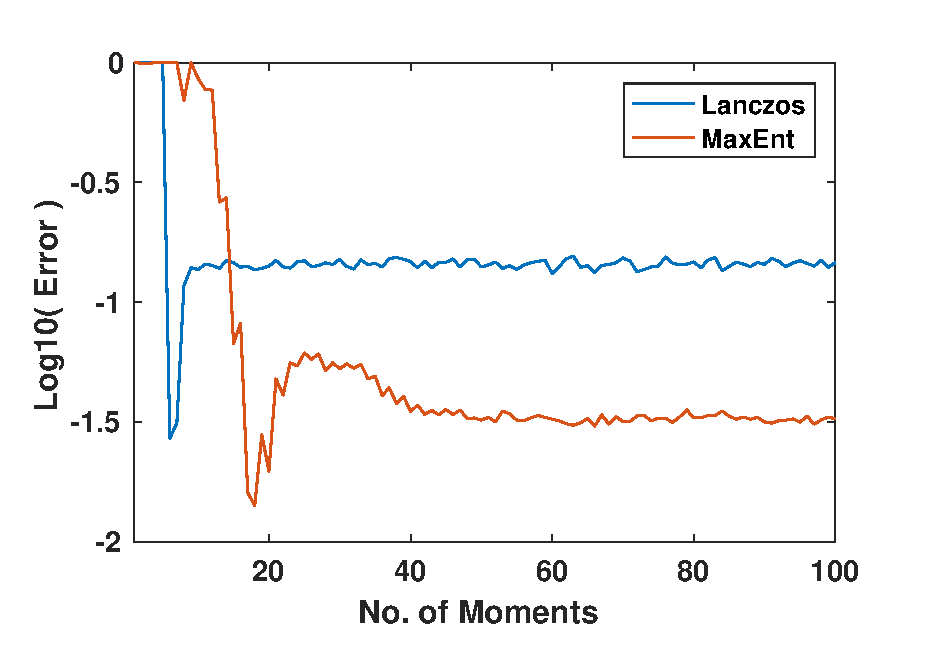
\includegraphics[trim=0.1cm 0cm 0.5cm 0.1cm, clip, width=1.0\linewidth]{Figures/Error_for_EmailL.eps}
		\caption{Email Dataset}
		\label{fig:emailerror}	
	\end{subfigure}%
	
	\begin{subfigure}
		\centering
		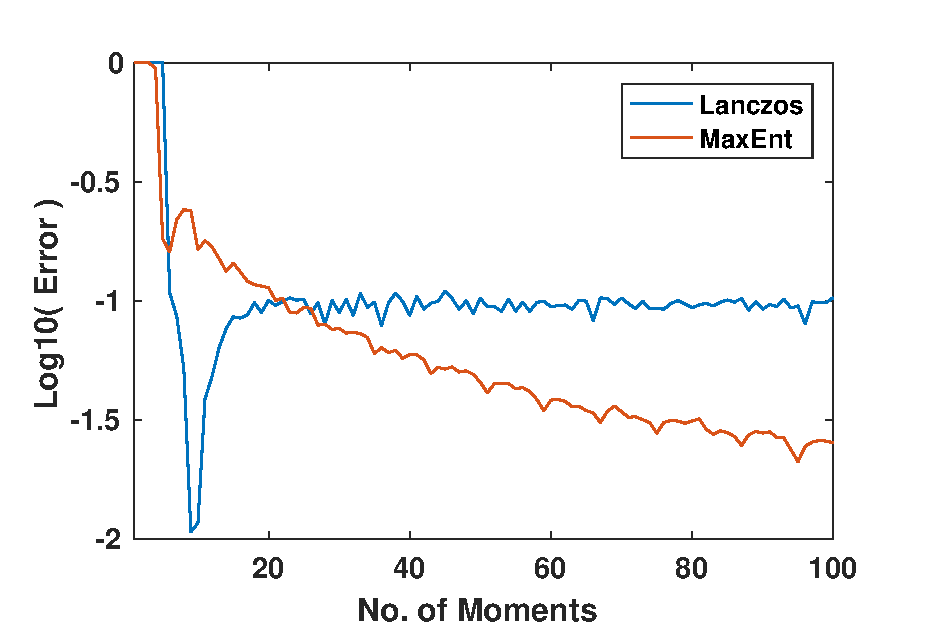
\includegraphics[trim=0.1cm 0cm 0.5cm 0.1cm, clip,  width=1.0\linewidth]{Figures/Error_for_NetscienceL.eps}
		\caption{NetScience Dataset}
		\label{fig:netscienceerror}
	\end{subfigure}
	\caption{Log error of community detection using MaxEnt and Lanczos algorithms on for differing number of moments $m$.}
	\label{fig:netscience}
\end{figure}

\label{smoothinglancsoz}
%We display the process of spectral learning for both MaxEnt and Lanczos, by plotting the spectral density of both methods against the true eigenvalue spectral density in Figure \ref{fig:emaildensity}. 
In order to make a valid comparison, we smooth the implied density using a Gaussian kernel, with $\sigma = 10^{-3}$. %We note that both MaxEnt and Lanczos approximate the ground truth better with a greater number of moments/steps $m$ and that Lanczos learns the extrema before the bulk of the distribution.
We plot the log error against the number of moments for both MaxEnt and Lanczos in Figure \ref{fig:emailerror}, with MaxEnt showing superior performance.
We repeat the experiment on the Net Science collaboration network, which represents a co-authorship network of $1,589$ scientists ($n = 1,589$) working on network theory and experiment \citep{newman2006finding}. The results in Figure \ref{fig:netscience} show that MaxEnt quickly outperforms the Lanczos algorithm after around $20$ moments.

% Acknowledgements should only appear in the accepted version.
\section{Appendix}
\subsection{First order Eigenvalue perturbation}

We formalise this intuition by considering a small perturbation of the Laplacian $\tilde{L} = L +\delta L$, where $|| \delta L|| \ll ||L||$. Considering the vectors $\vec{u_{i}}$ to be the normalised eigenvectors of the unperturbed Laplacian $L$ we solve the equation
\begin{equation}
(L+\delta L)(\vec{u_{i}}+\vec{\delta u_{i}}) = (\lambda_{i}+\delta\lambda_{i})(\vec{u_{i}}+\vec{\delta u_{i}})
\end{equation}
Cancelling and dropping second order terms we have
\begin{equation}
\label{firstorderterms}
\delta L \vec{u_{i}} + L\delta\vec{u_{i}}= \lambda_{i}\delta\vec{u_{i}} + \delta \lambda_{i}\vec{u_{i}}
\end{equation}
expressing the vector $\delta\vec{u_{i}}$ in the basis of the eigenvectors $\vec{u_{i}}$ of $L$, which can always be done as the $L$ is normal and hence its eigenvectors span the space of $\mathbb{R}^{n \times n}$, hence $\delta\vec{u_{i}} = \sum_{j}^{n}\epsilon_{j}\vec{u_{j}}$. Hence we can write equation \eqref{firstorderterms} as 
\begin{align}
& \delta L \vec{u_{i}} + L\sum_{j}^{n}\epsilon_{j}\vec{u_{j}}= \lambda_{i}\sum_{j}^{n}\epsilon_{j}\vec{u_{j}} + \delta \lambda_{i}\vec{u_{i}} \nonumber\\ 
%& \delta L \vec{u_{i}} + \sum_{j}^{n}\lambda_{j}\epsilon_{j}\vec{u_{j}}= \lambda_{i}\sum_{j}^{n}\epsilon_{j}\vec{u_{j}} + \delta \lambda_{i}\vec{u_{i}}\nonumber\\
& \vec{u_{i}}^{T}\delta L \vec{u_{i}} + \sum_{j}^{n}\lambda_{j}\epsilon_{j}\vec{u_{i}}^{T}\vec{u_{j}}= \lambda_{i}\sum_{j}^{n}\epsilon_{j}\vec{u_{i}}^{T}\vec{u_{j}} + \delta \lambda_{i}\vec{u_{i}}^{T}\vec{u_{i}}\nonumber\\
& \vec{u_{i}}^{T} \delta L \vec{u_{i}} = \delta \lambda_{i}
\end{align}
Where we have used the eigenvalue equation $L\vec{u_{i}} = \lambda_{i}\vec{u_{i}}$ and that the eigenvectors are orthonormal $\vec{u_{j}}^{t}\vec{u_{i}} = \delta_{i,j}$. We can now bound this term using the Cauchy-Schwarz inequality
\begin{equation}
\label{cauchyschwarz}
\delta \lambda_{i} =  \vec{u}_{i}^{T}\delta L \vec{u}_{i} \leq ||\delta L||\thinspace|| \vec{u}_{i}^{T}\vec{u}_{i}|| = ||\delta L||
\end{equation}

If we consider the natural variant of the Laplacian, normalised by the number of vertices in the graph, i.e $L_\mathrm{natural} = (D-A)/n$, then by adding $R$ vertices between previously disconnected subgraphs, for each vertex, we alter a two diagonal components by $+1$ and two off diagonal components by $-1$.Thus, using the Frobenius norm, our bound $B$ goes as
\begin{equation}
B = \sqrt{\sum_{i=1}^{n}\sum_{j=1}^{n}\bigg|\delta L_{i,j}\bigg|^{2}} = \frac{2R}{n}
\end{equation}
We note that our derived bound using the Cauchy-Schwarz inequality is exactly the same as Weyl's perturbation theorem for Hermitian matrices, which uses the min-max principle \citep{bhatia2013matrix}.


Hence we expect the eigenvalue perturbations to die off as $\mathcal{O}(n^{-1})$ for a constant number of connections between clusters as we increase the number of nodes $n$ in the network. Even if the number of such connections grows with $n$ but is sparse such that the total number is $\mathcal{O}(n s)$ with small sparsity $s$, the perturbation would only be of order $s$. For small sparsity $s$ we would expect the spectral gap between the perturbed eigenvalues which were at $0$ pre perturbation and the non zero eigenvalues to remain non-negligible. In these cases, we expect our cluster detection algorithm, introduced in the next section to also work.

If we choose to work with the normalised Laplacian defined in \eqref{lnorm}, then for each new connection between previously disconnected components we get a term of the form
%\begin{equation}
\begin{align}
& \sum_{j=1}\bigg|\bigg|\frac{1}{\sqrt{d_{i}d_{j}}}-\frac{1}{\sqrt{(d_{i}+1)d_{j}}}\bigg|\bigg|^{2}+\frac{2}{(d_{i}+1)(d_{k+1})} \nonumber \\
& + \sum_{l=1}\bigg|\bigg|\frac{1}{\sqrt{d_{k}d_{l}}}-\frac{1}{\sqrt{(d_{k}+1)d_{l}}}\bigg|\bigg|^{2}
\end{align}
%\end{equation}
where nodes $k$ and $i$ are being connected and nodes $j$ and $l$ are the nodes connected to $k$ and $i$, respectively. By taking the degrees to be a fraction of the total number of nodes $n$ and taking $n$ to be large we observed a similar $n^{-1}$ scaling. 
%%DO I NEED THIS SECTION?
The idea of strong communities being nearly disconnected components, is not novel \citep{mcgraw2008laplacian} and has been used in community detection algorithms \citep{capocci2005detecting}. However we have not come across a simple exposition of the results from matrix perturbation theory, or the application of the Cauchy-Schwarz inequality to bound the increase in the $0$ eigenvalues as a function of node number $n$ or degrees $d_{i}$ amongst the connected components.

\section{Polynomial approximations to the Log Determinant}
Recent work \cite{han2015large,dong2017scalable,zhang2007approximate} has considered incorporating knowledge of the non central moments \footnote{Also using stochastic trace estimation.} of a normalised eigenspectrum by replacing the logarithm with a finite polynomial expansion,
\begin{equation}
\label{polynomialexpansion}
\mathbb{E}_{\mu}  =  \int_{0}^{1}p(\lambda)\log (\lambda) d\lambda = \int_{0}^{1}p(\lambda)\log (1-(1-\lambda)) d\lambda.
\end{equation}
Given that $\log(\lambda)$ is not analytic at $\lambda = 0$, it can be seen that, for any density with a large mass near the origin, a very large number of polynomial expansions, and thus moment estimates, will be required to achieve a good approximation, irrespective of the choice of basis.

\subsection{Taylor approximations are probabilistically unsound}
\label{taylorisshit}
In the case of a Taylor expansion equation \eqref{polynomialexpansion} can be written as,
\begin{equation}
-\int_{0}^{1} p(\lambda)\sum_{i=1}^{\infty}\frac{(1-\lambda)^{i}}{i} \approx  -\int_{0}^{1} p(\lambda)\sum_{i=1}^{m}\frac{(1-\lambda)^{i}}{i}.
\end{equation}
The error in this approximation can be written as the difference of the two sums,
\begin{equation}
\label{taylorerror}
-\sum_{i=m+1}^{\infty}\frac{\mathbb{E}_{\mu}(1-\lambda)^{i}}{i},
\end{equation}
where we have used the Taylor expansion of $\log(1-x)$ and $\mathbb{E}_{\mu}$ denotes the expectation under the spectral measure.

De-Finetti \cite{finetti}  showed that Kolmogorov's axioms of probability \cite{kolmogorov_1950} could be derived by manipulating probabilities in such a manner so as to not make a sure loss on a gambling system based on them. Such a probabilistic framework, of which the Bayesian is a special case \cite{bayesianspecialcase}, satisfies the conditions of,
\begin{enumerate}
	\item \bfseries{Non Negativity:} $p_{i} \geq 0 \thinspace \forall i$,
	\item Normalization: $\sum_{i}p_{i} = 1$,
	\item Finite Additivity: $P(\cup_{n=1}^{N}A_{n}) = \sum_{n=1}^{N}P(A_{n})$.~~~\footnote{for a sequence of disjoint sets $A_{n}$.}
\end{enumerate}
The intuitive appeal of De-Finetti's sure loss arguments, is that they are inherently performance based. A sure loss is a practical cost, which we wish to eliminate. 

Keeping within such a very general formulation of probability and thus inference. We begin with complete ignorance about the spectral density $p(\lambda)$ (other than its domain $[0,1]$) and by some scheme after seeing the first $m$ non-central moment estimates we propose a surrogate density $q(\lambda)$. The error in our approximation can be written as,
\begin{eqnarray}
\label{spectralerror}
\int_{0}^{1} [p(\lambda)-q(\lambda)]\log(\lambda)d\lambda \nonumber \\
= \int_{0}^{1} -[p(\lambda)-q(\lambda)]\sum_{i=1}^{\infty}\frac{(1-\lambda)^{i}}{i}d\lambda.
\end{eqnarray}
For this error to be equal to that of our Taylor expansion \eqref{taylorerror}, our implicit surrogate density must have the first $m$ non-central moments of $(1-\lambda)$ identical to the true spectral density $p(\lambda)$ and all others $0$. %Given that we know that the spectral density $p(\lambda)$ is a sum of $n$ Dirac delta distributions with unknown locations\footnote
%{We could of course do $n$ sets of non central moment estimates using stochastic trace estimation and then solve for the location of the dirac delta functions exactly, however for a dense matrix this operation is $\mathcal{O}(n^{3})$ and hence no better than using the Cholesky decomposition so we are back where we started} bounded by the region $[0,1]$ the only case for which this is possible, would be for the $n$ delta distributions to co-locate at $\lambda=1$, This corresponds to the identity matrix, whose log determinant is trivially $0$ and the spectral expectation $E_{\mu}(1-\lambda)^{i} = 0,\thinspace \forall i$.

For any PD matrix $K$, for which $E_{\mu}(1-\lambda)^{i} > 0,\thinspace \forall i\leq m$\footnote{we except the trivial case of a Dirac distribution at $\lambda=1$, which is of no practical interest}, for equation \eqref{spectralerror} to be equal to \eqref{taylorerror}, we must have,
\begin{equation}
\int_{0}^{1}q(\lambda)\sum_{m+1}^{\infty}\frac{(1-\lambda)^{i}}{i}d\lambda = 0.
\end{equation}
Given that $ 0 \leq \lambda \leq 1$ and that we have removed the trivial case of the spectral density (and by implication its surrogate) being a delta function at $\lambda = 1$, the sum is manifestly positive and hence $q(\lambda) < 0$ for some $\lambda$, which is incompatible with the theory of probability \cite{finetti,kolmogorov_1950}.  

%In particular Determinental and Gaussian processes, for which their elegant probabilistic framework is regularly emphasised \cite{kulesza_2012,bauer2016understanding}, an approximation which violates the axioms of probability should be avoided.






\subsubsection{Prior Spectral Belief}
If we assume complete ignorance over the spectral domain, then the natural maximally entropic prior is the uniform distribution and hence $q(\lambda) = 1$.\footnote{Technically as the log determinant exists and is finite, we cannot have any mass at $\lambda=0$, hence we must set the uniform between some $[\delta\epsilon,1]$, where $\delta\epsilon >0$.}
An alternative prior over the $[0,1]$ domain is the Beta distribution, the maximum entropy distribution of that domain under a mean and log mean constraint,
\begin{equation}
\frac{\Gamma(\gamma+\beta)}{\Gamma(\gamma)\Gamma(\beta)}\lambda^{\gamma-1}(1-\lambda)^{\beta-1}.
\end{equation}
The log mean constraint is particularly interesting as we know that it must exists for a valid log determinant to exist, as is seen for equation \eqref{eq:spectrallog}.  We set the parameters of by maximum likelihood, hence,
\begin{equation}
\gamma = \frac{\mu_{1}(\mu_{1}-\mu_{2})}{\mu_{2}-\mu_{1}^{2}}\thinspace , \thinspace \beta = \bigg(\frac{1}{\mu_{1}}-1\bigg)\frac{\mu_{1}(\mu_{1}-\mu_{2})}{\mu_{2}-\mu_{1}^{2}}\thinspace.
\end{equation}

\subsubsection{Analytical surrogate form}
Our final equation for $q(\lambda)$ can be written as,
\begin{equation}
q(\lambda) = \frac{\Gamma(\gamma+\beta)}{\Gamma(\gamma)\Gamma(\beta)}\lambda^{\gamma-1}(1-\lambda)^{\beta-1}\times\exp(-[1+\sum_{i=0}^{m}\alpha_{i}\lambda^{i}])
\end{equation}
for the beta prior and 
\begin{equation}
q(\lambda) = \exp(-[1+\sum_{i=0}^{m}\alpha_{i}\lambda^{i}])
\end{equation}
for the uniform. The exponential factor can be thought of altering the prior beta/uniform distribution so as to fit the observed moment information. 



\section{Lagrangian Duality}
Consider a generic optimization problem of the form,
\begin{equation}
\begin{aligned}
&\text{minimize } \thinspace f_{0}(x)\\
&\text{subject to } \thinspace f_{i}(x) \leq 0, \thinspace i=1...m\\
&\text{subject to } \thinspace h_{i}(x) = 0, \thinspace i=1...p
\end{aligned}
\end{equation}
where $x \in \mathbb{R}^{n}$ and the domain $\mathcal{D} = \bigcap\limits_{i=0}^{m} f_{i}\cap\bigcap\limits_{i=1}^{p}h_{i}$. We define the Lagrangian dual function as the infimum of the Lagrangian over the domain of $x$,
\begin{equation}
\begin{aligned}
& g(\lambda,\nu) = \underset{x \in \mathcal{D}}{\inf}L(x,\lambda, \nu)\\
& = \underset{x \in \mathcal{D}}{\inf}\biggl( f_{0}(x) + \sum_{i=1}^{m}\lambda_{i}f_{i}(x) + \sum_{i=1}^{p}\nu_{i}h_{i}(x)\biggr).
\end{aligned}
\end{equation}
As the dual is the pointwise infimum of a family of affine functions of $(\lambda, \nu)$, it is concave, irrespective of the convexity of $f_{0},f_{i},h_{i}$. \cite{boyd_vandenberghe_2009}. It is easily verifiable due to the net negativity of the two summation terms in $g(\lambda, \nu)$ that the dual provides a lower bound on the optimal value $p^{*}$ of the primal problem. This is known as weak duality. In the case of equality constraints this bound is tight. 

For general inequality constraints the difference between the primal and dual optimal solution (duality gap) is not 0. However, for $f_{0}...f_{m}$ convex, affine equality constraints and certain regularity conditions, we have a duality gap of $0$, this is known as strong duality. An example of such a constraint qualification is Slater's condition, which states that there is an $x \in \textbf{relint } \mathcal{D}$ which satisfies the constraints.

\subsection{Application to Probability Distributions}
We consider a probability distribution $p:\mathcal{R}^{n} \rightarrow \mathcal{R}$ which satisfies the general axioms of non-negativity, associativity and normalizability. This defines a very general space of probability theories, of which the Bayesian formalism is a special case \cite{walley_1991}. Thus $p(x) \geq 0$ for all $x \in C$ and $\int p(x)dx = 1$, where $C \subseteq \mathcal{R}^{n}$ is convex. The last condition follows from the definition of convexity and the fact that any sum of two real numbers is a real number. Then as any non negative weighting of a convex set preserves convexity,
\begin{equation}
\int_{C}p(x)x\thinspace dx \in C \thinspace
\end{equation}
if the integral exists.

\subsection{Application to Maximum Entropy}
\label{entropydecreaseproof}
We wish to maximise the entropic functional $\mathcal{S}(p) = -\int p(x)\log p(x)dx$ under certain moment constraints $\int p(x)x^{m}dx = \mu_{m}$. This can be written as,
\begin{equation}
\begin{aligned}
&\text{minimize } \thinspace f_{0}[p(x)] = \int p(x)\log p(x)dx\\
&\text{subject to } \thinspace h_{i}[p(x)] = \int p(x)x^{i}dx - \mu_{i} = 0, \thinspace i=1...p.
\end{aligned}
\end{equation}
Given that the negative entropy is a convex objective and that the moment equality constraints are affine in the variable being optimised over $p(x)$ by strong duality we have an equivalence between the solution of the dual and that of the primal.

It is also clear that the domain defined as the intersection of the constraint sets can never increase upon the addition of an extra constraint. Hence,
\begin{equation}
\underset{x \in \mathcal{D}=\bigcap\limits_{i=0}^{m}f_{i}}{\inf}L(x,\lambda, \nu) \leq \underset{x \in \mathcal{D}=\bigcap\limits_{i=0}^{m+1}f_{i}}{\inf}L(x,\lambda, \nu)
\end{equation}
and thus the entropy can only decrease when adding an extra constraint. Hence by adding more moment constraints, we always reduce the entropy and given equations \eqref{dataprocessesing} and \eqref{sumentropies} we necessarily reduce $\mathcal{D}_{kl}(p(x)\|q(x))$, where $p(x), q(x)$ define the true eigenvalue and MaxEnt proposal distributions respectively

\section{KL as a measure of divergence}
Using Pinsker's inequality, which is tight up to constant factors, we can relate the KL divergence to both the total variation distance and the total variation norm \cite{cover2012elements}:
\begin{equation}
\delta(P,Q) \leq \sqrt{\frac{1}{2}\mathcal{D}_{kl}(P\|Q)},
\end{equation}
where the total variation distance is defined as
\begin{equation}
\delta(P,Q) = sup \{|P(A)-Q(A)|\} \text{where} \in \Sigma. 
\end{equation}
The total variation norm between $P$ and $Q$ can be written as,
\begin{equation}
|P-Q| \leq \sqrt{2\mathcal{D}_{kl}(P\|Q)}.
\end{equation}
This follows as $2\delta(P,Q) = |P-Q|_{1}$ where the 1 relates to the $L{1}$ norm.

\section{Bound on Error of MaxEnt}
To calculate the log determinant of the matrix in question, once we have the proposal eigenvalue distribution $q(x)$ we calculate the mean value of $\log(x)$ under the distribution $q(x)$, i.e $\int q(x)\log(x)dx$. We can write the error of our MaxEnt estimate as
\begin{equation}
\epsilon = \biggl| \int_{x\in \chi}[p(x)-q(x)]\log(x)dx\biggr|
\end{equation}
Where $p(x)$ is the true eigenvalue distribution. $\forall p(x),q(x) \geq 0$ it is hence true that,
\begin{equation}
\biggl|\int_{x\in \chi}(p(x)-q(x))\log(x)dx\biggr| \leq  \int_{x\in \chi} |p(x)-q(x)||\log(x)| dx.
\end{equation}
From the monotonicity of the function $\log(x)$, we have that  $\log(x) \leq \mbox{max}[|\log(x_{max})|,|\log(x_{min})|$ and rewriting the total variational norm in terms of the KL divergence we have:
\begin{equation}
\label{errorequation}
\epsilon \leq \mbox{max}[|\log(x_{max})|,|\log(x_{min})|]\sqrt{2\mathcal{D}_{kl}(P\|Q)}.
\end{equation}
We thus note that by reducing the self entropy of the proposal distribution $q(x)$ we necessarily reduce the maximum possible error of the log determinant estimation. However, given that we do not have an analytic form of $p(x)$, we cannot explicitly calculate $\mathcal{D}_{kl}(P\|Q)$ and hence the bound in its current form is not inherently practical. We leave the estimation of this term and derivation of estimate uncertainty to future work.

Conditions for the existence of a solution to this problem have been proved for the case of the Hausdorff moment conditions \cite{mead1984maximum}, of which our problem is a special case.

\begin{figure}
	\begin{subfigure}%{width=0.2\textwidth}
		\centering
		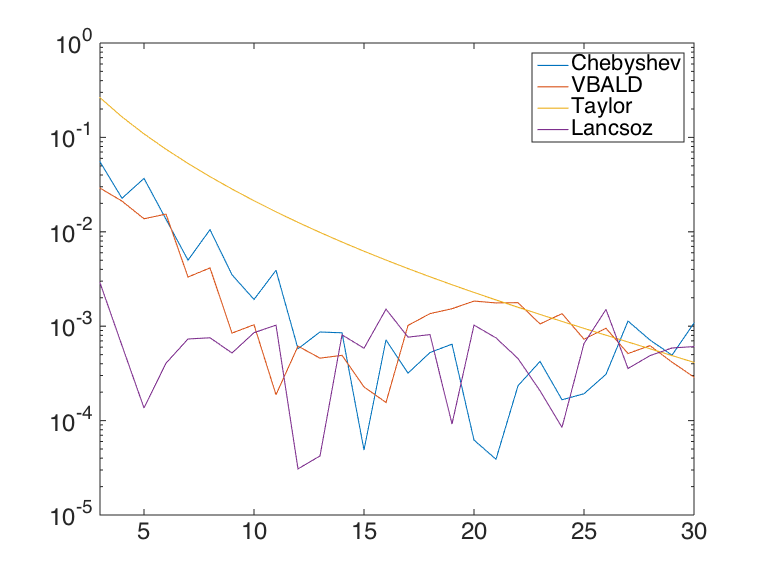
\includegraphics[width=1\linewidth]{propercond30dim0p1}
		\caption{Length Scale = 0.1, Condition number = 16}
		\label{fig:lscale0.1}
	\end{subfigure}
	\begin{subfigure}%{.2\textwidth}
		\centering
		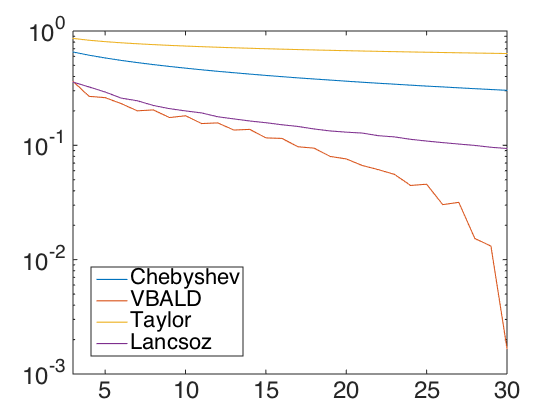
\includegraphics[width=1\linewidth]{69500756condl0p33}
		\caption{Length Scale = 0.33, Condition number = $2\times 10^{7}$ Equivalent Chebyshev steps $n=1200$, Lanczos steps $n\approx 100$.}
		\label{fig:lscale0.33}
	\end{subfigure}
	\caption{Comparison of MaxEnt against Taylor, Lanczos and Chebyshev algorithms for calculating the log determinant of synthetic squared exponential kernel matrices of different condition number. The absolute relative error is on the $y$-axis and number of moments used on the $x$-axis.}
\end{figure}

\section*{Acknowledgements}




% In the unusual situation where you want a paper to appear in the
% references without citing it in the main text, use \nocite

\bibliography{sample}
\bibliographystyle{aaai}
\end{document}
